\documentclass{article}


\usepackage[margin=1.2in]{geometry}
\usepackage{parskip}

\relax % Controls
    \newif\ifmarginprooflinks
    	\marginprooflinkstrue
    	% \marginprooflinksfalse

\relax % Bibliography, etc
	\usepackage[american]{babel}
	\usepackage{csquotes}
	\usepackage[backend=biber, style=authoryear]{biblatex}
	\DeclareLanguageMapping{american}{american-apa}
	% \usepackage[backend=biber,style=authoryear,hyperref=true]{biblatex}
	% \addbibresource{refs.bib}
	% \addbibresource{conf.bib}

	\DeclareFieldFormat{citehyperref}{%
	  \DeclareFieldAlias{bibhyperref}{noformat}% Avoid nested links
	  \bibhyperref{#1}}

	\DeclareFieldFormat{textcitehyperref}{%
	  \DeclareFieldAlias{bibhyperref}{noformat}% Avoid nested links
	  \bibhyperref{%
	    #1%
	    \ifbool{cbx:parens}
	      {\bibcloseparen\global\boolfalse{cbx:parens}}
	      {}}}

	\savebibmacro{cite}
	\savebibmacro{textcite}

	\renewbibmacro*{cite}{%
	  \printtext[citehyperref]{%
	    \restorebibmacro{cite}%
	    \usebibmacro{cite}}}

	\renewbibmacro*{textcite}{%
	  \ifboolexpr{
	    ( not test {\iffieldundef{prenote}} and
	      test {\ifnumequal{\value{citecount}}{1}} )
	    or
	    ( not test {\iffieldundef{postnote}} and
	      test {\ifnumequal{\value{citecount}}{\value{citetotal}}} )
	  }
	    {\DeclareFieldAlias{textcitehyperref}{noformat}}
	    {}%
	  \printtext[textcitehyperref]{%
	    \restorebibmacro{textcite}%
	    \usebibmacro{textcite}}}

	\DeclareCiteCommand{\brakcite}
	  {\usebibmacro{prenote}}
	  {\usebibmacro{citeindex}%
	   \printtext[bibhyperref]{[\usebibmacro{cite}]}}
	  {\multicitedelim}
	  {\usebibmacro{postnote}}

\relax % Standard Packages
    \usepackage[dvipsnames]{xcolor}
    % \usepackage[utf8]{inputenc}
    \usepackage{mathtools}
    \usepackage{amssymb}
		\DeclareMathSymbol{\shortminus}{\mathbin}{AMSa}{"39}
    % \usepackage{parskip}
    % \usepackage{algorithm}
    \usepackage{bbm}
	\usepackage{lmodern}
	% \usepackage{times}
    \usepackage{faktor}
    % \usepackage{booktabs}
	% \usepackage[margin=1in]{geometry}
    \usepackage{graphicx}
    \usepackage{scalerel}
    \usepackage{enumitem}
    \usepackage{nicefrac}\let\nf\nicefrac

    % \usepackage{color}
    %\usepackage{stmaryrd}
    \usepackage{hyperref} % Load before theorems...
        \hypersetup{colorlinks=true, linkcolor=blue!75!black, urlcolor=magenta, citecolor=green!50!black}

\usepackage{tikz}
	\usetikzlibrary{positioning,fit,calc, decorations, arrows, shapes, shapes.geometric}
	\usetikzlibrary{cd}

	%%%%%%%%%%%%
	\tikzset{AmpRep/.style={ampersand replacement=\&}}
	\tikzset{center base/.style={baseline={([yshift=-.8ex]current bounding box.center)}}}
	\tikzset{paperfig/.style={center base,scale=0.9, every node/.style={transform shape}}}

	% Node Stylings
	\tikzset{dpadded/.style={rounded corners=2, inner sep=0.7em, draw, outer sep=0.3em, fill={black!50}, fill opacity=0.08, text opacity=1}}
	\tikzset{dpad0/.style={outer sep=0.05em, inner sep=0.3em, draw=gray!75, rounded corners=4, fill=black!08, fill opacity=1, align=center}}
	\tikzset{dpadinline/.style={outer sep=0.05em, inner sep=2.5pt, rounded corners=2.5pt, draw=gray!75, fill=black!08, fill opacity=1, align=center, font=\small}}

 	\tikzset{dpad/.style args={#1}{every matrix/.append style={nodes={dpadded, #1}}}}
	\tikzset{light pad/.style={outer sep=0.2em, inner sep=0.5em, draw=gray!50}}

	\tikzset{arr/.style={draw, ->, thick, shorten <=3pt, shorten >=3pt}}
	\tikzset{arr0/.style={draw, ->, thick, shorten <=0pt, shorten >=0pt}}
	\tikzset{arr1/.style={draw, ->, thick, shorten <=1pt, shorten >=1pt}}
	\tikzset{arr2/.style={draw, ->, thick, shorten <=2pt, shorten >=2pt}}

	\newcommand\cmergearr[5][]{
		\draw[arr, #1, -] (#2) -- (#5) -- (#3);
		\draw[arr, #1, shorten <=0] (#5) -- (#4);
		}
	\newcommand\mergearr[4][]{
		\coordinate (center-#2#3#4) at (barycentric cs:#2=1,#3=1,#4=1.2);
		\cmergearr[#1]{#2}{#3}{#4}{center-#2#3#4}
		}
	\newcommand\cunmergearr[5][]{
		\draw[arr, #1, -, shorten >=0] (#2) -- (#5);
		\draw[arr, #1, shorten <=0] (#5) -- (#3);
		\draw[arr, #1, shorten <=0] (#5) -- (#4);
		}
	\newcommand\unmergearr[4][]{
		\coordinate (center-#2#3#4) at (barycentric cs:#2=1.2,#3=1,#4=1);
		\cunmergearr[#1]{#2}{#3}{#4}{center-#2#3#4}
		}

\usepackage{amsthm,thmtools} % Theorem Macros
	\usepackage[noabbrev,nameinlink,capitalize]{cleveref}
    \theoremstyle{plain}
    \newtheorem{theorem}{Theorem}
	\newtheorem{coro}{Corollary}[theorem]
    \newtheorem{prop}[theorem]{Proposition}
    \newtheorem{conj}[theorem]{Conjecture}
    \newtheorem{claim}{Claim}
    \newtheorem{remark}{Remark}
    \newtheorem{lemma}[theorem]{Lemma}
    \theoremstyle{definition}
    % \newtheorem{defn}{Definition}
    % \declaretheorem[name=Definition]{defn}
    \declaretheorem[name=Definition, qed=$\square$]{defn}
    \declaretheorem[name=Example, qed=$\triangle$]{example}

    \definecolor{openQcolor}{rgb}{0.9,0.2,0.9}
    \declaretheorem[preheadhook=\color{openQcolor},name=Open Question]{openQ}

	\crefname{defn}{Definition}{Definitions}
	\crefname{prop}{Proposition}{Propositions}
    \crefname{issue}{Issue}{Issues}

\relax %%%%%%%%% GENERAL MACROS %%%%%%%%
    \let\Horig\H
	\let\H\relax
	\DeclareMathOperator{\H}{\mathrm{H}} % Entropy
	\DeclareMathOperator{\I}{\mathrm{I}} % Information
	\DeclareMathOperator*{\Ex}{\mathbb{E}} % Expectation
	\DeclareMathOperator*{\EX}{\scalebox{1.5}{$\mathbb{E}$}}
    \newcommand{\ifrac}[2]{{#1}/{#2}}
    
    % \DeclareMathOperator{\argmin}{\arg\min}
    \DeclareMathOperator*{\argmin}{\arg\!\min}
    \DeclareMathOperator*{\argmax}{\arg\!\max}

    \newcommand{\mat}[1]{\mathbf{#1}}
    \DeclarePairedDelimiterX{\infdivx}[2]{(}{)}{%
		#1\;\delimsize\|\;#2%
	}
	\newcommand{\thickD}{I\mkern-8muD}
	\newcommand{\kldiv}{\thickD\infdivx}
	\newcommand{\tto}{\rightarrow\mathrel{\mspace{-15mu}}\rightarrow}

	\newcommand{\datadist}[1]{\Pr\nolimits_{#1}}
	% \newcommand{\datadist}[1]{p_\text{data}}

	\makeatletter
	\newcommand{\subalign}[1]{%
	  \vcenter{%
	    \Let@ \restore@math@cr \default@tag
	    \baselineskip\fontdimen10 \scriptfont\tw@
	    \advance\baselineskip\fontdimen12 \scriptfont\tw@
	    \lineskip\thr@@\fontdimen8 \scriptfont\thr@@
	    \lineskiplimit\lineskip
	    \ialign{\hfil$\m@th\scriptstyle##$&$\m@th\scriptstyle{}##$\hfil\crcr
	      #1\crcr
	    }%
	  }%
	}
	\makeatother
	\newcommand\numberthis{\addtocounter{equation}{1}\tag{\theequation}}

\relax %%%%%%%%%   PDG  MACROS   %%%%%%%%
	\newcommand{\ssub}[1]{_{\!_{#1}\!}}
	% \newcommand{\bp}[1][L]{\mat{p}_{\!_{#1}\!}}
	% \newcommand{\bP}[1][L]{\mat{P}_{\!_{#1}\!}}
	\newcommand{\bp}[1][L]{\mat{p}\ssub{#1}}
	\newcommand{\bP}[1][L]{\mat{P}\ssub{#1}}
	\newcommand{\V}{\mathcal V}
	\newcommand{\N}{\mathcal N}
	\newcommand{\Ed}{\mathcal E}

    \newcommand{\balpha}{\boldsymbol\alpha}
    \newcommand{\bbeta}{\boldsymbol\beta}

	\DeclareMathAlphabet{\mathdcal}{U}{dutchcal}{m}{n}
	\DeclareMathAlphabet{\mathbdcal}{U}{dutchcal}{b}{n}
	\newcommand{\dg}[1]{\mathbdcal{#1}}
	\newcommand{\PDGof}[1]{{\dg M}_{#1}}
	\newcommand{\UPDGof}[1]{{\dg N}_{#1}}
	\newcommand\VFE{\mathit{V\mkern-4mu F\mkern-4.5mu E}}

	\newcommand\Inc{\mathit{Inc}}
	\newcommand{\IDef}[1]{\mathit{IDef}_{\!#1}}
	% \newcommand{\ed}[3]{%
	% 	\mathchoice%
	% 	{#2\overset{\smash{\mskip-5mu\raisebox{-3pt}{${#1}$}}}{\xrightarrow{\hphantom{\scriptstyle {#1}}}} #3} %display style
	% 	{#2\overset{\smash{\mskip-5mu\raisebox{-3pt}{$\scriptstyle {#1}$}}}{\xrightarrow{\hphantom{\scriptstyle {#1}}}} #3}% text style
	% 	{#2\overset{\smash{\mskip-5mu\raisebox{-3pt}{$\scriptscriptstyle {#1}$}}}{\xrightarrow{\hphantom{\scriptscriptstyle {#1}}}} #3} %script style
	% 	{#2\overset{\smash{\mskip-5mu\raisebox{-3pt}{$\scriptscriptstyle {#1}$}}}{\xrightarrow{\hphantom{\scriptscriptstyle {#1}}}} #3}} %scriptscriptstyle
	\newcommand{\ed}[3]{#2%
	  \overset{\smash{\mskip-5mu\raisebox{-1pt}{$\scriptscriptstyle
	        #1$}}}{\rightarrow} #3}

    \newcommand{\nhphantom}[2]{\sbox0{\kern-2%
		\nulldelimiterspace$\left.\delimsize#1\vphantom{#2}\right.$}\hspace{-.97\wd0}}
		% \nulldelimiterspace$\left.\delimsize#1%
		% \vrule depth\dp#2 height \ht#2 width0pt\right.$}\hspace{-.97\wd0}}
	\makeatletter
	\newsavebox{\abcmycontentbox}
	\newcommand\DeclareDoubleDelim[5]{
	    \DeclarePairedDelimiterXPP{#1}[1]%
			{% box must be saved in this pre code
				\sbox{\abcmycontentbox}{\ensuremath{##1}}%
			}{#2}{#5}{}%
		    %%% Correct spacing, but doesn't work with externalize.
			% {\nhphantom{#3}{##1}\hspace{1.2pt}\delimsize#3\mathopen{}##1\mathclose{}\delimsize#4\hspace{1.2pt}\nhphantom{#4}{##1}}
			%%% Fast, but wrong spacing.
			% {\nhphantom{#3}{~}\hspace{1.2pt}\delimsize#3\mathopen{}##1\mathclose{}\delimsize#4\hspace{1.2pt}\nhphantom{#4}{~}}
			%%% with savebox.
		    {%
				\nhphantom{#3}{\usebox\abcmycontentbox}%
				\hspace{1.2pt} \delimsize#3%
				\mathopen{}\usebox{\abcmycontentbox}\mathclose{}%
				\delimsize#4\hspace{1.2pt}%
				\nhphantom{#4}{\usebox\abcmycontentbox}%
			}%
	}
	\makeatother
	\DeclareDoubleDelim
		\SD\{\{\}\}
	\DeclareDoubleDelim
		\bbr[[]]
	% \DeclareDoubleDelim
	% 	\aar\langle\langle\rangle\rangle
	\makeatletter
	\newsavebox{\aar@content}
	\newcommand\aar{\@ifstar\aar@one@star\aar@plain}
	\newcommand\aar@one@star{\@ifstar\aar@resize{\aar@plain*}}
	\newcommand\aar@resize[1]{\sbox{\aar@content}{#1}\scaleleftright[3.8ex]
		{\Biggl\langle\!\!\!\!\Biggl\langle}{\usebox{\aar@content}}
		{\Biggr\rangle\!\!\!\!\Biggr\rangle}}
	\DeclareDoubleDelim
		\aar@plain\langle\langle\rangle\rangle
	\makeatother


	% \DeclarePairedDelimiterX{\aar}[1]{\langle}{\rangle}
	% 	{\nhphantom{\langle}{#1}\hspace{1.2pt}\delimsize\langle\mathopen{}#1\mathclose{}\delimsize\rangle\hspace{1.2pt}\nhphantom{\rangle}{#1}}

\relax %%%%% restatables and links
	% \usepackage{xstring} % for expandarg
	\usepackage{xpatch}
	\makeatletter
	\xpatchcmd{\thmt@restatable}% Edit \thmt@restatable
	   {\csname #2\@xa\endcsname\ifx\@nx#1\@nx\else[{#1}]\fi}% Replace this code
	   % {\ifthmt@thisistheone\csname #2\@xa\endcsname\typeout{oiii[#1;#2\@xa;#3;\csname thmt@stored@#3\endcsname]}\ifx\@nx#1\@nx\else[#1]\fi\else\csname #2\@xa\endcsname\fi}% with this code
	   {\ifthmt@thisistheone\csname #2\@xa\endcsname\ifx\@nx#1\@nx\else[{#1}]\fi
	   \else\fi}
	   {}{\typeout{FIRST PATCH TO THM RESTATE FAILED}} % execute on success/failure
	\xpatchcmd{\thmt@restatable}% A second edit to \thmt@restatable
	   {\csname end#2\endcsname}
	   {\ifthmt@thisistheone\csname end#2\endcsname\else\fi}
	   {}{\typeout{FAILED SECOND THMT RESTATE PATCH}}

	% \def\onlyaftercolon#1:#2{#2}
	\newcommand{\recall}[1]{\medskip\par\noindent{\bf \Cref{thmt@@#1}.} \begingroup\em \noindent
	   \expandafter\csname#1\endcsname* \endgroup\par\smallskip}

   	\setlength\marginparwidth{1.55cm}
	\newenvironment{linked}[3][]{%
		\def\linkedproof{#3}%
		\def\linkedtype{#2}%
		% \reversemarginpar
		% \marginpar{%
		% \vspace{1.1em}
		% % \hspace{2em}
		% 	% \raggedleft
		% 	\raggedright
		% 	\hyperref[proof:\linkedproof]{%
		% 	\color{blue!50!white}
		% 	\scaleleftright{$\Big[$}{\,{\small\raggedleft\tt\begin{tabular}{@{}c@{}} proof of \\\linkedtype~\ref*{\linkedtype:\linkedproof}\end{tabular}}\,}{$\Big]$}}
		% 	}%
        % \restatable[#1]{#2}{#2:#3}\label{#2:#3}%
		\ifmarginprooflinks
		\marginpar{%
			% \vspace{-3em}% %% for bottom
			\vspace{1.5em}
			\centering%
			\hyperref[proof:\linkedproof]{%
            % \hyperref[proof:#3]{
			\color{blue!30!white}%
			\scaleleftright{$\Big[$}{\,\mbox{\footnotesize\centering\tt\begin{tabular}{@{}c@{}}
				% proof of \\\,\linkedtype~\ref*{\linkedtype:\linkedproof}
				link to\\[-0.15em]
				proof
			\end{tabular}}\,}{$\Big]$}}~
			}%
		\fi
        \restatable[#1]{#2}{#2:#3}\label{#2:#3}%
        }%
		{\endrestatable%
		}
	\makeatother
		\newcounter{proofcntr}
		\newenvironment{lproof}{\begin{proof}\refstepcounter{proofcntr}}{\end{proof}}

		\usepackage{cancel}
		\newcommand{\Cancel}[2][black]{{\color{#1}\cancel{\color{black}#2}}}

		\usepackage{tcolorbox}
		\tcbuselibrary{most}
		\tcolorboxenvironment{lproof}{
			% fonttitle=\bfseries,
			% top=0.5em,
			enhanced,
			parbox=false,
			boxrule=0pt,
			frame hidden,
			borderline west={4pt}{0pt}{blue!20!black!40!white},
			% coltext={blue!20!black!60!white},
			colback={blue!20!black!05!white},
			sharp corners,
			breakable,
			% bottomsep at break=4cm,
			% enlarge bottom at break by=-4cm,
			% topsep at break=3cm,
			% enlarge top at break by=-3cm
		}
		% \usepackage[framemethod=TikZ]{mdframed}
		% \surroundwithmdframed[ % lproof
		% 	   topline=false,
		% 	   linewidth=3pt,
		% 	   linecolor=gray!20!white,
		% 	   rightline=false,
		% 	   bottomline=false,
		% 	   leftmargin=0pt,
		% 	   % innerleftmargin=5pt,
		% 	   skipabove=\medskipamount,
		% 	   skipbelow=\medskipamount
		% 	]{lproof}
	%oli16: The extra space was because there was extra space in the paragraph, not
	%because this length was too big. By breaking arrays, everything will be better.
	\newcommand{\begthm}[3][]{\begin{#2}[{name=#1},restate=#3,label=#3]}

\relax %TODOs and footnotes
    \newcommand{\TODO}[1][INCOMPLETE]{{\centering\Large\color{red}$\langle$~\texttt{#1}~$\rangle$\par}}
    \newcommand{\dfootnote}[1]{%
        \let\oldthefootnote=\thefootnote%
        % \addtocounter{footnote}{-1}%
		\setcounter{footnote}{999}
        \renewcommand{\thefootnote}{\textdagger}%
        \footnote{#1}%
        \let\thefootnote=\oldthefootnote%
    }
	\newcommand{\dfootnotemark}{
		\footnotemark[999]
	}


% \usepackage[framemethod=TikZ]{mdframed}
% \colorlet{color1}{Emerald}
% \colorlet{color3}{color1>wheel,2,3}
% \colorlet{pinkish}{color3!25!magenta}
\definecolor{brownish}{rgb}{0.5, 0.2, 0.1}
% \newmdenv[roundcorner=5pt, 
%     backgroundcolor=brownish!20!white,
%     % frametitle={$\langle$under construction$\rangle$},
%     frametitle={$\langle$incomplete or buggy$\rangle$},
%     frametitlerule=false,
%     innertopmargin=3pt, frametitlebelowskip=1ex, frametitleaboveskip=1ex,
%     frametitlebackgroundcolor=brownish!40!white,
%     skipabove=1em,skipbelow=1em,
%     frametitlefont={\scshape},leftmargin=-10pt, rightmargin=-10pt]
% 		{wip}
\newtcolorbox{wip}{%
    colback=brownish!20!white,%
    % frametitle={$\langle$under construction$\rangle$},
    title={$\langle$under construction$\rangle$},%
    enhanced jigsaw,
    breakable,
    % frametitlerule=false,
    % innertopmargin=3pt, frametitlebelowskip=1ex, frametitleaboveskip=1ex,
    colframe=brownish!40!white,%
    % skipabove=1em,skipbelow=1em,
    % frametitlefont={\scshape},leftmargin=-10pt, rightmargin=-10pt
}
        
% \tcolorboxenvironment{example}{
% \newtcolorbox[use counter=example]{examplex}{
\newtcbtheorem[use counter=example]{examplex}{Example}{
        label type=example,
        fonttitle=\bfseries,
        % empty,
        enhanced jigsaw,
        % title={Example \thetcbcounter.},
        before=\par\medskip\noindent,
        % top=0.5em,
        % enhanced,
        parbox=false,
        % boxrule=0pt,
        % frame hidden,
        % borderline west={4pt}{0pt}{green!20!black!40!white},
        % coltext={blue!20!black!60!white},
        % colback={blue!20!black!05!white},
        colback=white,
        sharp corners,
        breakable,
        % bottomsep at break=4cm,
        % enlarge bottom at break by=-4cm,
        % topsep at break=3cm,
        % enlarge top at break by=-3cm
    }
    %
    {ex}


\makeatletter
\newcommand{\@minipagerestore}{\setlength{\parskip}{\medskipamount}}
\makeatother

\usepackage{xparse}
\let\realItem\item % save a copy of the original item
\makeatletter
\NewDocumentCommand\myItemboldperiod{ o }{%
   \IfNoValueTF{#1}%
      {\realItem}% add an item
      {\realItem[\textbf{#1.}]\def\@currentlabel{#1}%
        % \def\cref@currentlabel{#1}
        }% add an item and update label
}
\makeatother


% \usepackage{enumitem}
\newlist{URaxioms}{enumerate}{1}
\setlist[URaxioms]{
    resume,%
    label=\textbf{UR\arabic{*}.},
    % label=UR\arabic{*},
    ref={UR\arabic*},
    leftmargin=2cm,
    before=\let\item\myItemboldperiod,
    topsep=1ex
    }
% \crefname{URaxiomsi}{axiom}{axioms}
\crefname{URaxiomsi}{}{}
\newcommand\commentout[1]{}

\addbibresource{conf.bib}

\usepackage{booktabs}

\newcommand{\ext}[1]{\overline #1} %  measures over phi
\newcommand{\Unif}{\mathrm{Unif}}

\def\cofunc{commitment function}
\def\confdom{\mathdcal C}
\def\ZO{\mathrm{ZO}}
% \def\ZO{[0,1]}
\def\Rplus{\mathbb R_+}

% \let\oldTheta\Theta
% \renewcommand\Theta{\mathdcal{\Theta}}

% \title{Measures of Confidence}
\title{Updating With Confidence}
\author{Oliver E Richardson, Joseph Y Halpern}

\begin{document}
\maketitle

\tableofcontents
\clearpage

\section{Introduction}

\def\stmt{$A$}
% \def\stmt{$\phi$}

% The ability express information with varying confidence is an important aspect of knowledge representation.
% Being able to articulate things with variable confide

The ability articulate a ``degree of confidence'' is an important aspect of knowledge representation.
% We give a formal account of a new concept
% We are about to propose a concept . 
% Subpoint: it helps avoid a brittleness of always beliving things
% Subpoint: Protects against overconfidence.
Of course, there are many well-established ways of representing uncertainty,
	probability chief among them.
	% and chief among them is probability.
% probability chief among them. 
% Indeed, an informal poll of our colleagues suggests that computer scientists use ``confidence'' as a synonym for probability.
% The concept is so dominant that an informal poll of our colleagues suggests that most computer scientists view ``confidence'' as a synonym for probability.
Indeed, an informal poll of our colleagues suggests that most computer scientists view ``confidence'' as a synonym for probability.
% In our view, this practice 
Although this use of the word is perfectly reasonable, it seems to have shadowed another conception of confidence---one that is fundementally different, if at first sublty so. 
% which seems have been shadowed by the enormous success of probability---one that is fundementally different, if at first subtly so.
% which seems to have been shadowed by the enormous success of probability---a concept that is fundementally different, if at first subtly so.
 
% , such as belief functions, and most importantly, probabilities.
% In each case, one adopts a more complex belief state, 
% The enormous success of probability in particular has had an enormous impact on the way computer scientists talk about 
% The success of probability has shadowed other concepts that might well also be called measures of confidence.
% Indeed, it 

% There are actually two related, but slightly different notions here. 
% % The first is a measurement of
% There is a second setting in which one might interpret the word confidence, as well, in an updating context: it's how seriously you take an input 
% Note the difference: 




For us, confidence is a measure of trust. 
Like probability, it is a scale between two extremes. 
% While probability ranges from untenable (0) to undeniable (1),
While probability ranges from untenable (0) to undeniable (1),
confidence ranges from completely untrustworthy $(\bot)$ to fully trusted ($\top$). 
%
% We apply this notion confidence of updating.
% This paper explores how confidence works in state-updating context.
This paper explores how confidence works in the context of learning.
In this setting, one has some belief state, and recieves inputs, which one might have some degree of confidence in, which is used to modify one's belief state. 
Our use of confidence can be viewed as a measure of how seriously to take an input in updating our beliefs.

High confidence is in many ways like high probability: if we really trust a statement \stmt, we should fully incorporate it into our beliefs, and thereby come to believe it with high probability. 
Similarly, it only makes sense to be extremely confident in a \stmt\ if you believe that \stmt\ is extremely likely to be true. 
Low confidence, on the other hand, is quite different from low probability. 
If we have little trust in \stmt, we should \emph{ignore} \stmt, rather than coming to believe that \stmt\ is unlikely.
% To say \stmt\ has low probabilty is  high confidence in the $\lnot$\stmt. 
For example, if an adversary tells you something that you happen to already believe,
% is likely to be true
you might say you have low confidence in their statement, but nevertheless ascribe it high probability. 

% The approach we take in this paper is very general, 
% Our approach is quite general, and applies any time a belief state is modified in resonse to an input. 
% one wants to measure (gradual) incorporation of new information into one's beliefs, and may be thought of as a measure of how much of the new information makes it into one's beliefs. 


\subsection{Other Conceptions of Confidence.}

\textbf{Probability.}
% Probability is a numerical scale that ranges from untenable (0) to undeniable (1). 
% No number on this scale is truly neutral.
% One of the biggest shortcomings of probability is its inability to represent a truly neutral attitude towards a proposition.  
Some people do use ``confidence'' to mean the same thing as probability. When they say they have low confidence in $\phi$, they mean that they think $\phi$ is unlikely. 

One of the biggest shortcomings of probability is its inability to represent a truly neutral attitude towards a proposition.  
%  probability of $\frac12$ .
% This shortcoming has perhaps been the primary selling point of many alternatives to probabiltiy, such as Dempster-Shafer Belief functions. 
A value of $\frac12$ may be equally far from zero as it is from one, but is by no means a neutral assessment in all cases: hearing that your favored candidate has a 50\% chance of winning is big news if a win was previously thought to be inevitable. 
For this reason, telling someone the odds are 50/50 is quite different from saying you have no idea. 
% By contrast, zero confidence represents a truly neutral stance; a statement with zero confidence has no effect.  
By contrast, zero confidence represents something truly neutral: 
	a statement made with zero confidence does not stake out a claim, and 
	a statement recieved with zero confidence does not affect the recipient's beliefs. 
Nevertheless, in some contexts, we will see that confidences correspond to to probabilities.

\textit{Opacity.} To use a graphical metaphor, think of certainty as black or white.
Probability describes shades of gray, while confidence describes opacity. 
If we are painting with black and start with a white canvas, there is a precise correspondence between the opacity and the resulting shade of gray.

\textbf{Upper and Lower Probabilities.}
Upper and lower probabilities can describe a neutral attitude towards a proposition, but they are not really a specification of trust, but rather a direct specification of a belief state. 
It isn't immediately clear how to use these representations of uncertainty to update, and they're a little too complex to function effectively as the primitive measure of trust that we're after.


\textbf{Shafer's Weight of Evidence.}
Shafer's ``weight of evidence'' is precisely the same concept we have in mind. 
Our analysis precsely reduces to his, in the setting where belief states are Belief functions (which generalize probabilities, but not, say, neural network weights), and observations are events. 
% This paper can be a generalization of Shafer's ``weight of evidence'' to a broader class of settings, where one might have very different belief states and observations. 
Thus, this paper can be viewed as generalizing this concept to a broader class of settings, without requiring that one adopt Shafer's conception of a belief state or an observation. 


\textbf{Variance and Entropy.}
The inverse of variance, sometimes known as precision,
	is also commonly used to measure confidence. 
If a sensor is unreliable and can give a range of answers, the variance of the estimate is a very common way of quantifying this reliablility.
If measurements have zero variance, in some sense one has absolute confidence ($\top$) in the sensor. If measurements have infinite variance, then in some sense one has no confidence in the sensor, since individual samples convey no information about the true value of the quantity measured.
As with probability, inverse variance will coincide with confidence in some settings; we will see how in \cref{sec:variance}.

Entropy, like variance, is a standard way of measuring uncertainty, and in some settings, confidence coincides with entropy (see \cref{sec:entropy}).
The assumption underlying both approaches is that there's some ``true'' value of the variable, and that the randomness is epsistemic (due to sensor errors) rather than aleotoric (inherrent in the quantity being measured). 

\textbf{Confidence Intervals and Error Bars.}
Another notion of the word ``confidence'' comes from the term ``confidence interval''.
This concept arises in settings involving a probability distribution $\Pr(X)$ over a metric space $X$, typically $X = \mathbb R$. 
A 95\% confidence interval is the (largest) ball containing 95\% of the probability, and its size is a geometric measurement of how . 
This intuition behind this reading of the word confidence is the same as  

% For example, suppose we recieve an input \stmt.  If we completely trust \stmt, we should integrate it fullly into our beliefs.  Thus, the effect of having high confidence in \stmt\ is that we come to believe \stmt\ with high probability.
% If we know that the input comes from an untrustworthy source, for instance, the best thing to do is to ignore it entirely, even if 

% because we want to be able to deal with information that we aren't certain about.

%
% It is extremely useful to be able to express variable confidence in information
%%
%%
%%
% Among computer scientists, the notions of confidence and probability are often identified.
% Among computer scientists, ``confidence'' is often a synonym for probability.
% % ---%
% % Although the two notions are closely related, it is important to distinguish between confidence and likelihood.
% For instance, it is common to say that one has ``high confidence in a statement \stmt'' to indicate a belief that
% % (the content of) \stmt is likely to be true.
% \stmt\ is likely to be true.
% But
% % However,
% having high confidence in \stmt\ can also mean something subtly different: that we should \emph{trust} \stmt, in the sense of taking it seriously in updating our beliefs.
% % The two notions might seem indistinghishable at first,
% % This distinction may not at first seem meaningful, because if we take \stmt\ seriously in updating our beliefs, we will ultimately believe \stmt\ is likely.
% If we take \stmt\ seriously in updating our beliefs, we will ultimately believe \stmt\ is likely, and so the distinction might not seem meaningful at first.
% % However, the two are quite different at the other end of the spectrum. If you believe that \stmt\ is
% % However, thinking that one should \emph{not} trust \stmt\ is quite different from thinking that \stmt\ is unlikely.
% % But \emph{low} probability is quite different from low probability.
% % At the other end of the scale, however, the two notions differ a great deal.
% But at the other end of the scale, the two notions are quite different.
% If we have little trust in \stmt, we should \emph{ignore} \stmt, rather than coming to believe that \stmt\ is unlikely.
% So, if an untrusted party tells you something that you happen to already believe, you might reasonably ascribe it high probability but low confidence.

% We argue that confidence is a useful concept, distinct from probability.
% We will show how confidences
% In this paper, we give a formal framework for talking about confidence in the context of updating,
% which we then use to interperet quantities across a wide variety of settings as confidences.
% % In each case, we will see the following features:

% \subsection{Recurring Themes}
% Here are some recurring themes:
% 
% \begin{enumerate}[nosep]
%     \item Updating with zero confidence leaves the belief state unchanged.
%     \item Updating with absolute certainty (the limit as confidence becomes large) causes you to (permanently) gain a certainty, and acts like a projection.
%     % \item A zero-confidence update does nothing, while
%     % \item Zero confidence is neutral.
%     % updating with certainty (the limit of large confidence) is a projection.
%     % \item Updating with certainty (the limit of large confidence) is a projection.
%     \item Confidence measures involve an arbitrary choice of scale, and so only ratios of confidences are meaningful.
%     % \item $\exp(- \beta E)$
%     % \item Confidence tends to end up as the scaling term for an exponential functions
%     % \item Update rules are exponential in confidence.
% \end{enumerate}


% Theorem. Certainties can never be gained or lost with any finite sequence of differentiable updates.
% Theorem. Certainty is always infinitely far away, as measured by the Riemannian metric.

% \section{Update Rules}
\section{A Formalism for Updating}
\def\X{\mathcal X}
\def\W{\mathcal W}

% The setup is as follows.
Suppose you you have some belief state $\theta \in \Theta$. 
% $\Theta$ might be \textellipsis
% \begin{itemize}[nosep]
%     \item $\Delta W$, the set of probability distributions over measurable space $W$ of outcomes;
%     \item the set of parameters to some parametric family of distributions;
%     \item the set of belief functions over a common space of outcomes;
%     \item the set of all possible PDGs;
%     \item a set of worlds an agent considers possible;
%     \item 
% \end{itemize}
It might be 
a probability distribution, a parameter setting to some parameteric family of probabilities, a set of probabilities, a Dempster-Shafer belief function, or even just a setting of weights for a neural network. 
Now, suppose you recieve some input information $\phi \in \Phi$, such as an event, or a sample from a dataset, which you may use to update your belief state. 
%
% Before we add confidence into the mix, let's first see how this setup works without it, so that we can more clearly see what is missing.
Before we get to confidence, let's first see how far we can get without it.
% The first assumption we make is that the updating process can be captured in functional form. 
The first thing we need to assume is that the updating process can be captured in functional form. 
% The primary assumption that we have to make is:
\begin{CFaxioms}
	\item[\textbf{F}] 
		% The updating process can be described as a function 
		There exists a function
		% $F : \Theta \times \Phi \to \Theta$,
		$F : \Phi \to ( \Theta \to \Theta)$,
		which, given the old belief state $\theta$ and new information $\phi$, produces the belief state $F_\phi\theta$ that corresponds to the result of observing $\phi$ in state $\theta$.
		% which produces a new belief state, as a function of the old belief state and the new information.
\end{CFaxioms}

% In some ways this seems very reasonable: 
Given such a function $F$ and a statement $\phi$, we call $F_\phi : \Theta \to \Theta$ an \emph{update}. 
% At this point, since we have no way of articulating how confident we are in the new information, the only reasonable thing to 
At face value, \textbf{F} seems very reasonable: what more could your next belief state depend on, aside from your previous one and the new information? 
Nevertheless, we will soon argue that the resulting belief state $\theta'$ should also depend on something else: one's confidence in the statement.
 % after which we will weaken \textbf{F} appropriately.

In any case, since the purpose of $F$ is to \emph{fully} incorporate the new information into our beliefs
(and without a notion of confidence, we can't very well specify how much to incorporate), then
% it should be the case that a second update with the same information should not affect the belief state.
% a second update with the same information should not affect the belief state.
two successive updates with the same information ought to have the same effect as a single one.
Intuitively, this is because if we have just \emph{fully} updated our beliefs to be consistent with the information $\phi$, then a second observation of $\phi$ will require no further alterations of our belief state.
In this case, we call $F$ an \emph{update rule}, or more precisely, a \emph{$\Theta$-update rule on $\Phi$}, and insist that
\begin{CFaxioms}
	\item[\textbf{UR}] For all $\phi \in \Phi$, the update $F_\phi$ is
	% require that it be idempotent.
	idempotent (i.e., $F_\phi \circ F_\phi = F_\phi$).
\end{CFaxioms}

% In curried form, $F : \Phi \to (\Theta \to \Theta)$. 

% We now proceed with the formal details.
% \textbf{Update Rules.}
% Consider a space $\Theta$
% of possible belief states,
% and a set $\Phi$ of statements.
% % and a set $\Phi$ of ``statements'', i.e., the things one can have confidence in.
% % An \emph{update rule} (or more precisely, a \emph{$\Theta$-updating rule on $\Phi$})
% An \emph{update rule}, or more precisely, a \emph{$\Theta$-update rule on $\Phi$},
% is a function of the form
% \[
%     % F :  (\mathbb R \times \Phi) \to \Big( \Theta \to \Theta \Big)
%     F :  \Phi \to \Big( \Theta \to \Theta \Big)
% \]
% % which describes how to update beliefs about $X$, with the new information, at a certain level of trust.
% which describes how to (fully) update beliefs $\Theta$ with new information $\Phi$.
% and for $F$ to be an update rule, we require that , meaning that updating any belief with $\phi$ twice in a row is equivalent to single update.
% Having said that, one reading of this paper is a relaxation of this requirement.
% Here are some examples.
Once $\Theta$, $\Phi$, and any implicit structure in them is specified, there is typically a natural choice of update rule. 
To illustrate, we now consider three different probability-update rules for different choices of $\Phi$.
In each case, the possible belief states $\Theta := \Delta W$ be the set of all probability distributions over a finie set $W = \{w_1, \ldots, w_n\}$ of ``possible worlds''. 

\begin{enumerate}
	\item %\textbf{Conditioning.}
	\textbf{Conditioning.}
	First, consider the case where observations are events, i.e., $\Phi := 2^W$. 
	% One particularly natural $\Delta W$-update rule on $2^W$ is given by conditioning,
	% Here, the appropriate update seems to be condition:
	Here, the appropriate rule seems to be conditioning:
	\[
	\begin{aligned}
		(-) \smash{\,\Big|\,} (\;\cdot\;) : \qquad 2^W &\to (\Delta W \to \Delta W) \\
		% (-) \smash{\,\Big|\,} (\;\cdot\;) : \qquad 2^W \times \Delta W &\to \Delta W \\
		% (-) \,\Big|\, (\;\cdot\;) : \Delta X \times 2^X \to \Delta X.
		% (\mu \in \Delta X, A \subset X) &\mapsto \mu | A .
		% (A \subset W) &\mapsto (  ~~\mu~~ \mapsto \mu \mid A ),
		A  &\mapsto (  ~\mu~~ \mapsto \mu \mid A ~),
		% (A, \mu) ~&\mapsto~  \mu \mid A\, ,
	\end{aligned}
	% \qquad
	% \qquad
	% \begin{tikzpicture}[center base]
	%     \node[dpad0] (W) {$W$};
	%     \node[dpad0, right=0.5 of W] (Aq) {$A?$};
	%     \draw[arr2, <-] (W) to node[above]{$\mu$} ++(-1, 0);
	%     \draw[arr2, ->>] (W) to node[above,pos=0.3]{} (Aq);
	%     \draw[arr2, <<-] (Aq) to node[above,pos=0.7]{$A!$} ++(1.2,0);
	% \end{tikzpicture}
	\]
	% where $(\mu \mid A)(x) = \frac{\mu(\{x\})}{\mu(A)}$
	% in which learning $A$ maps
	% where the action of the conditional measure $\mu\mid A$ is given by $(\mu \mid A) \{w\} = \ifrac{\mu\{w\}}{\mu(A)}$.
	% where the action of the conditional measure $\mu\mid A$ is given by $(\mu \mid A)(B) = \ifrac{\mu(B \cap A)}{\mu(A)}$, provided $\mu(A) > 0$,
	where the conditional measure $\mu\mid A$ is given by $(\mu \mid A)(B) = \ifrac{\mu(B \cap A)}{\mu(A)}$, provided $\mu(A) > 0$,
	% and may be defined arbitrarily otherwise.
	and otherwise is just equal to $\mu$.
	Observe:
	\begin{itemize}[nosep]
		\item Provided $\mu(A) > 0$, then $(\mu\mid A) \mid A = \mu \mid A$, so conditioning is an update rule.
		\item If $\mu(A \cap B) > 0$, then $(\mu \mid A) \mid B = \mu \mid (A \cap B) = (\mu \mid B) \mid A$, so the order that information is recieved does not matter, so long as that information is consistent with one's beliefs.
	\end{itemize}
	% However, it is not the only $\Delta W$-updating rule for $2^W$.
	 % $\Phi$.

	\item
	\textbf{Imaging.}
	A second example of an update rule is the ``imaging'' approach of David Lewis
	\parencite{lewis1976probabilities}.
	% , albeit in very different notation.
	% Once again, consider a finite set $W$, and belief states $\Theta := \Delta W$.
	Suppose that, for some set $\Phi$, that we already have a $W$-update rule
	$f : \Phi \to (W \to W)$, which we interpret as assigning, to each statement $\phi \in \Phi$ and $w \in W$, a unique world $f_\phi w \in W$ which is the world ``most similar to $w$, in which $\phi$ is true'' \parencite{gardenfors1979imaging}.
	In this case, idempotence of $f_\phi$ amounts to the (very reasonable) requirement that the world most similar to $f_\phi w$ in which $\phi$ is true, is $f_\phi w$ itself.
	From $f$, we can construct a $\Delta W$-update rule by
	\[
	\begin{aligned}
		F_\phi(\mu) &:=
			f^{\sharp}(\mu) \\
			% &= A \mapsto \mu( f^{-1}_\phi( A ))\\
			&= A \mapsto \mu(\{w : f(w) \in A\})
	\end{aligned}
		\qquad
		\qquad
		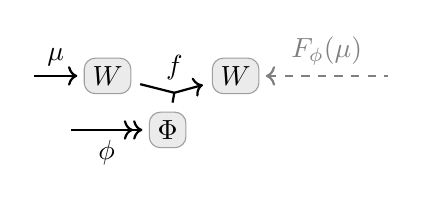
\begin{tikzpicture}[center base]
			\node[dpad0] (W) {$W$};
			\node[dpad0, right=1 of W] (W') {$W$};
			\node[dpad0, below right=0.2 and 0.2 of W] (Phi) {$\Phi$};
			\mergearr{W}{Phi}{W'}
			\node[above=1pt of center-WPhiW']{$f$};
			\draw[arr2, <-] (W) to node[above]{$\mu$} ++(-1, 0);
			\draw[arr2, <<-] (Phi) to node[below]{$\phi$} ++(-1.3, 0);
			\draw[arr2, <-, dashed, gray] (W') to node[above]{$F_\phi(\mu)$} ++(2, 0);
		\end{tikzpicture}
	\]
	which intuitively moves the probability mass on each world $w$ to the $f_\phi w$, the closest world to $w$ in which $\phi$ is true.
	% is the pushforward measure of $\mu$ through $f_\phi$, which Lewis calls the ``image of $\mu$ on $\phi$''
	And, since $f$ is idempotent, $F$ will be as well.


	\commentout{
	\item More generally, consider a measurable space $\W = (W, \mathcal A)$, where $W$ is a set and $\mathcal A$ is a $\sigma$-algebra over $W$, and let $\mathcal F \subset \mathcal A$ be closed under supersets in $\mathcal A$.
	% Now, let $\Theta$ be the set of conditional probabili$

	\TODO[Properly Use Conditional Probability Measure, to define on all events]

	Conditioning a probability distribution $\mu \in \Delta\X$ on an event $A \in \mathcal A$ also makes sense in this more general measure-theoretic setting, at least so long as $\mu(A) > 0$, and is given by
	% the Lebesgue integral
	% \[
	$$
		% (\mu \mid A) (B) = \frac{1}{\mu(A)} \int \mathbf 1_{B}(x)  \mathrm d\mu(x)
		(\mu \mid A) (B) = \frac{\mu(B \cap A)}{\mu(A)}
	$$
	}


	\item \textbf{Jeffrey's Rule.}
	% Once more, suppose that $W$ is a finite set and $\Theta := \Delta W$.
	Next, consider a more general form of observation, in which observations themselves are probabilities. 
	% Formally, suppose $\Phi$ consists of pairs $(X,\pi)$,
	% Formally, suppose $\Phi$ consists of marginal distributions $\pi(X)$
	Formally, suppose $\Phi$ consists of distributions $\pi(X)$,
	% written $\pi(X)$,
	where $X : W \to S$ is a random variable,
	% (i.e., some function of $W$),
	and $\pi \in \Delta S$ is a distribution over the possible values that $X$ can take.
	Jeffrey's rule, given by
	\begin{align*}
		% \mathrm{Jeffrey}_{(X,\pi)}
		% \mathrm{Jeffrey}_{\pi(X)}
		\mathrm{J}_{\pi(X)}
		(\mu) &:= \sum_{x \in S} \pi(X\!=x) \;  \mu \,\Big|\, \{ w : X(w) = x \}
			\\
			&= A \mapsto \sum_{x \in S} \pi(X\!=x)\, \mu( A \mid X \!= x)
	\end{align*}

	When $\pi(X) = \delta_x$ is a point mass $X=x$, then Jeffrey's Rule simply conditions on the event $X = x$.
	 % but for other choices of $\pi(X)$,
	For this reason, Jeffrey's Rule is sometimes seen as a way of making an update with uncertainty (i.e., a ``low-confidence'' update), but as we will see, it instead is perhaps better thought of as a high-confidence update on a more expresive class of observations.
	
	Note that if $\mu' := J_{\pi(X)}\mu$ is the result of applying Jeffrey's rule to $\pi(X)$ and $\mu$, 
	% then $\pi$ will be fully incorporated (that is, $\mu'(X) = \pi(X)$), 
	then $\mu'(X) = \pi(X)$, so $\pi(X)$ has been fully incorporated into $\mu'$, and the old beliefs $\mu(X)$ about $X$ have been completely destroyed by the update.
\end{enumerate}




% , at a certain level of trust.
% We are interested in . A \emph{}
% Each of these update rules takes its 
If we take a step back, fully incorporating information is really quite extreme. 
% For agents that uses conditioning, for instance, incorporation is permanent. 
% Observing information 
An agent that updates with conditioning for instance, is forever committed to fully believing $A$, and consequently, learns nothing from observing $A$ agin in the future. 
Humans don't work this way. 
The effectiveness of flash cards as a learning tool demonstrates this clearly:
if we were using an update rule, two cycles through a deck of flash cards would be no different from one.
Similarly, artificial neural networks are trained with many incremental updates, and cycle through training data more than once.
Indeed, this is one biggest differences between modern machine learning algorithms and the older rule-based ones: the new ones update parameters little-by-little, rather than fully incorporating input information.
% Once an agent that uses conditioning incorporates $A$, it is forever committed to believing $A$, and as a side effect, there is no point to making 
How shall we alter our picture to account for less extreme belief alterations, in which information is only partially incorporated?
This is where confidence comes in. 
% This is where other value confidence comes in. 
% Humans don't always update our beliefs with update functions.
% Often there seems to be value in learning the same thing more than once---or, put another way---in updating with confidence.


% To that end, we now consider a domain of possible values of confidence, which describes a degree of incorporation.
% To that end,


% We now define a \emph{\cofunc} to be a function

Let $\confdom$ be the set of possible confidences, which, for now, we will take to be the interval $[0, 1]$. 
% We are now in a position to consider confidence when updating. 
We are now in a position to take confidence into account in our updates. 
As before, our first axiom is that we can capture the updating process in functional form. 

\begin{CFaxioms}
	\item[CF0] 
	There exists some function 
	% $F : \Theta \times \Phi \to \Theta$,
	\[
		F : \confdom \to ( \Phi \to ( \Theta \to \Theta) )
	\]
	which, given a confidence and new information $\phi$, in addition to a prior belief state $\theta$, produces the belief state $F^c_\phi\theta$ that corresponds to the result of observing $\phi$ in state $\theta$. \label[CFaxiomsi]{ax:funcform}
\end{CFaxioms}

% Although not incontrovertable, this seems like a reasonable requirement.  
% After all, if 
% Although not incontrovertable, this seems like a reasonable requirement.
% It is not so important that the function be deterministic---we can make it a non-deterministic or probabilistic without too much hassle---the real purpose of \cref{ax:funcform} is to assert that all of the information we need to compute the next belief state is contained in either
% % (1) our previous belief state, (2) the new information, or (3) our confidence in it.
% in our prior belief state $(\theta)$, the new information $(\phi)$, or our attitude towards it ($c$).

Historically speaking, \cref{ax:funcform} has not proved as anodyne as it looks. 
Some might object that it's not possible to write such a function that is appropriate in all circumstances.
For example, Shafer argues for Dempster's rule of combination as a way of incorporating information, but is very careful to emphasize that it ought to be used only on \emph{independent} information, for reasons illustrated below. 



\begin{example}\label{ex:dupl}
	You have initial belief state $\theta_0$.
	Now, someone comes up to you and tells you that $\phi$ is true, a statement
		that you trust to some intermediate degree of confidence $c \notin\{ \bot, \top\}$. 
	So, in accordance with \Cref{ax:funcform}, you use $F$ to transform your beliefs, partially incorporating the information to arrive at some belief state $\theta_1 := F^c_\phi(\theta_0)$.
	Immediately afterwards, your friend repeats what they just said: $\phi$ is true. 
	Your confidence in the statement remains the same, and so according to 
	\Cref{ax:funcform}, you again update your beliefs, arriving at $\theta_2 := F^c_\phi(\theta_1)$. 
	Except in very special circumstances (e.g., you already know that $\phi$ is true, or $c \in \{\bot,\top\}$), typically $\theta_2$. 
	And yet, it seems your your attitude towards $\phi$ ought to be the same whether you've heard it twice or only once.
\end{example}


Now, it's important to mention that we're not quite in the same position as Shafer.
Shafer was prescribing a concrete representation of $\Theta$ (a belief function) and a concrete update rule $F$ (Dempster's rule of combination), and so he needed to defend these choices. 
% To take an analogous prescriptive stance,
We only need to defend something much more modest: we only need to defend the assumption that, if $\Theta$ and $\Phi$ properly model the relevant aspects of the scenario at hand, then there exists \emph{some} function $F$ which performs updates appropriately. 
Descriptively speaking, we're also in good shape: for synthetic agents, it suffices to point out that learning algorithms represent functions, which given a state, an input, and a number of iterations (confidence), produce an output. 
And, supposing that $\Theta$, $\Phi$, and $\confdom$ all capture the relevant respective aspects of a human's belief state, input information, and attitude towards it, how could it be that a human does otherwise?
%
% After all, if you recieve the same input twice, and your confidence in it has not changed, it would be best to only update once. 
% There are essentially three ways to proceed.
In any case, keeping \cref{ex:dupl} in mind, here are three ways to proceed.

\begin{enumerate}[label={\textbf{I\arabic*.}},ref={I\arabic*}]
	\item \textbf{Accept Severe Limiations.} \label{approach:assume}
	Like Shafer, we could be careful 
	% not to claim anything about how to update beliefs, except
	to claim nothing about the belief updating process except in the (unusual) case where 
	information recieved is independent.
	% This severly handicaps the usefulness of . 
	This would be a severe limiation to the theory, and much less necessary than it was for Shafer. 
	Imagine that we are writing code that describes how a synthetic agent updates its beliefs. Shafer's approach is to package any such code with a warning against running it unless assured that observations will always be independent. 
	But independece is notoriously difficult to establish; are we to simply accept that the code will not behave correctly in any realistic scenario?
	% Under what circumstances could we possibly be sure that all inputs we will be independent?    
	
	In practice, many theoretical properties of standard statistical learning algorithms are heavily dependent on indepencence assumptions (most commonly, that one recieves independent, identically distributed samples).
	% Despite this, such algorithms .
	This warning label not seem to keep them from being applied in settings where practitioners readily admit samples are not really independent at all---nor indeed performing well emperically in those settings \parencite{???}.

	% If we need to make a decision that depends on information that is not given, then     
	% Shafer found himself in a position where he needed to qualify usage of the update rule
	
	
	\item \textbf{Appropriately Enrich Domains.}\label{approach:enrich}
	% For instace, the agent has been totally 
	% We told a story wanting to avoid incorporating information twice. 
	In \cref{ex:dupl}, it seems obvious that we ought to ignore the second copy of the information, because it has already been accounted for.
	However, this intuition is highly contingent on the implicit supposition that we \emph{know} the second input to be a replica of the first.
	Were we ignorant to the nature of the second piece of information, perhaps it would not be so unreasonable to incroproate it again, even without a proof of independence. 
	% If we want our agent to do the same
	% In asking our agent to take such issues into account, it is only fair to give it access to the same 
	% It seems unfair to criticize an agent for not behaving 
	So, if we would like our agent to make the same decisions that we did, it seems only fair to give it access to the knowledge that we needed to get there. 
	One way of doing this is to extend the belief state so that it also tracks what information has been incorporated.  
	% For instance, suppose that every message 
	
	For \cref{ex:dupl} to work, it is critical that we are able to discern that the two inputs were identical.
	As a result, it seems that the relevant description of the input information was not just $\phi$, but a pair $(\phi, \mathit{id})$ that also a description of its identity.
	It is also critical that we remember the identity of previously incorporated information, so we would also be better off with a belief space $\Theta$ reflects this.  
	With these two modifications, any \cofunc\ can be straightforwardly modified to avoid the issue in \Cref{ex:dupl}. 

	
	We submit that it is always possible to enrich the space of beliefs and observations in this way to track the relevant information, to resolve the issue.
	With a few more assumptions later on, we will be able to formalize the construction we just alluded to (\cref{ex:dupl-enriched}).

	\item \textbf{An Incremental Interpretation of Confidence.}
		\label{approach:interperet}
	Finally, we can get around the issue by interpreting a confidence $c \in \confdom$ not as an absolute measurement of confidence, but rather an incremental one.  This means viewing $c \in \confdom$ as the degree of \emph{additional} confidence we have in $\phi$, beyond whatever we have already incorporated into our beliefs. 
	
	% This proposal immediately raises some important questions.
	This proposal might be concerning.
	% First, how 
	One might worry that it's harder to make sense of ``incremental confidence'' than an absolute notion.
	How ought we to numerically describe the confidence of an update? 
	Suddenly this becomes much more subjective, for to assign a number, not only must we describe how much trust we have in the new information, but we must also take history or current belief state into account.
	Furthermore, the words ``incremental'' and ``additional'' suggest that we will need a formal description of how to aggregate confidences---%
	the very concept of which we will need to defend.
	% Indeed, such a way of combining confidences will ultimately play a large role for us. 
	% It will turn out that such a way of combining confidences 
	% Fortunately, it will turn out that 

	Even modulo these concerns, the incremental interpretation still leaves us in a strictly better place than we were before.
	%  with \cref{approach:assume}.
	To begin, in situations where inputs are independent (i.e., the only cases where we would have been allowed to apply the \cofunc\ according to \cref{approach:assume}), the two notions coincide. 
	More explicitly: if the new information $\phi$ is indepenendent of everything we've previously seen, then an absolute measurement of our confidence in it is no different from a measrurement of how much we ought to increment it from having no confidence.
	Already, though, we can do more.
	In the situation described by \cref{ex:dupl}, for instance, 
	the second utterance induce no \emph{additional} confidence ($\bot$), and so applying $F$ with no confidence clearly gives the desired result of ignoring the new information (per \cref{ax:zero}). 
%
%
	And even in general, the prospect of having to numerically estimate a fuzzy quantity seems more promising than red tape requiring that $F$ only be used (in good conscience) on independent information.	
	% In some ways, this approach it is not so different from directly requiring independence of inputs, there are several aspects of this framing, that in our view, make it more pallatable.    
	% First, 
	% In cases
	% This raises some questions. Even if we already had a 

\end{enumerate}


% We submit that any information that is relevant to that final belief state ought to be present in one of these places. For instance, if we've already heard this same information before, this fact should either be present in our beliefs $(\theta)$, in the observation $(\phi)$, or in the description of our confidence in it ($c$).


% which, given an incremental confidence $c \in \mathbb \confdom$, returns an ``incremental'' update rule, i.e., a function with the same type as an update rule, except possibly non-idempotent.
% which, given a confidence $c \in \mathbb \confdom$, returns an ``incremental'' update rule,
% i.e., a function with the same type as an update rule, except possibly not idempotent.
% i.e., a function $F^c : \Phi \to (\Theta \to \Theta)$ that may not be idempotent.
Given a confidence $c \in \confdom$ and a statement $\phi \in \Phi$, we write
 % Given a piece of information $\phi \in \Phi$, , we write
% $F^\beta_\phi : \Delta\X \to \Delta X$
$F^c_\phi : \Theta \to \Theta$
for the update prescribed by the \cofunc\ $F$.
% Furthermore, we will insist that \cofunc s .
Furthermore, we will insist that \cofunc s respect our interpretation of confidence at the two extremes.
% , especially the following two.
\begin{CFaxioms}
	% \item \textbf{(zero)} $F^{0}_A(\Pr) = (\Pr)$
	% \item  $F^{0}_A  = {1}_{\Delta\X}$. (That is, $F^{0}_A(\Pr) = \Pr$ for all $\Pr \in \Delta\X$.)
	% \item  $F^{0}_\phi  = {1}_{\Delta\X}$. (That is, $F^{0}_\phi(\Pr) = \Pr$ for all $\Pr \in \Delta\X$.)
	%     \hfill \textbf{(zero)} \label{ax:zero}
	\item 
		% $F^{\bot}_\phi  = {\mathrm{Id}}_{\Theta}$.\\
		% (That is, $F^{\bot}_\phi(\theta) = \theta$ for all $\theta \in \Theta$.)
		For all $\theta \in \Theta$ and $\phi \in \Phi$, $F^{\bot}_\phi(\theta) = \theta$.
		% \hfill \textbf{(no confidence)} \label{ax:zero}
		% \hfill \textbf{(zero)} \label{ax:zero}
		\hfill \textbf{(neutrality)} \label{ax:zero}
	% \item $F^{\beta_1}_A \circ F^{\beta_2}_A = F^{\beta_1 + \beta_2}_A$
	% \item $F^{\top} : \Phi \to (\Theta \to \Theta)$ is an update rule, i.e.,
	%     the funciton $F^{\top}_\phi : \Theta \to \Theta$ is an idempotent.
	\item
		% For all $\phi$,
		For all $\phi$,
		% $F^\top_\phi$
		$F^\top_\phi : \Theta \to \Theta$
		is an idempotent update.\\
		Equivalently, $F^\top: \Phi \to (\Theta \to \Theta)$ is an update rule.
		% the funciton $F^{\top}_\phi : \Theta \to \Theta$ is an idempotent.
% If $F$ is a \cofunc, then by \cref{ax:idemp}, $F^{\top}$ is an update rule, and we call $F$ a ``refinement'' of the update rule $F^{\top}$.
		\hfill \textbf{(certainty)} \label{ax:idemp}\\
		We call $F$ a \emph{refinement} of the update rule $F^\top$.
% \end{CFaxioms}
% The next axiom,
% \begin{CFaxioms}
	% \item For all $\beta_1, \beta_2 \in \mathbb R_{\ge 0}$,~
	% 
	% \item For all $c_1, c_2 \in \confdom$,~
	%     $F^{c_1}_\phi \circ F^{c_2}_\phi = F^{c_1 \oplus c_2}_\phi$
	%     % \hfill \textbf{(additivity)} \label{ax:additivity}
	%     \hfill \textbf{(combination)} \label{ax:additivity}
\end{CFaxioms}
\Cref{ax:zero} captures the intuition that we should ignore information in which we have no confidence, while \cref{ax:idemp} formalizes the intuition that a full-confidence updates act as we imagined.
At this point, we would like to point out that those who find \cref{ax:zero} reasonable have implicitly either accepted either \cref{approach:assume} or \cref{approach:interperet}.

\begin{example}
	Suppose you first hear $\phi$ from a partially trusted source, and incroproate it into your beliefs appropriately.  
	Then, the same source sends you a second message, which is obviously spam.
	In an absolute sense, you now have no confidence ($\bot$) in anything this source tells you, including (in retrospect) both messages. 
	It seems appropriate to excise $\phi$ from your belief state in response, rather than leaving your belief state unchanged, as \cref{ax:zero} would prescribe. 

	Note that in this scenario, while it seems that we ultimately have no confidence in $\phi$, it does not seem to be the case that we have no incremental confidence in $\phi$.  
	Rather, the incremental confidence seems to be the inverse of the original confidence.  
\end{example}

From this point forward, we use the incremental interpretation of confidence, with the understanding that it also admits a more conservative reading (in that it is less widely applicable), in which confidence is measured absolutely, and also all applications of the function $F$ are independent. 


% \Cref{ax:additivity} states that, for all $\theta$, the function $c \mapsto F^c_\phi\theta : \confdom \to \Theta$ is a group homomorphism.
 % a confidence of $\top$ indicates that we are fully incorporating information into our beliefs.




\begin{phaseout}
and so for most of this paper, we take $\confdom := \Rplus$ to be the group of extended nonnegative real numbers under addition.
With this choice of confidence domain, \cref{ax:additivity} begins to have more bite, although, as we will see, the effect is more to pin down a coherent system of measurement, and does not appear to restrict modeling expressivness.
%
%
% Below is a concrete representative example of a \cofunc\ with our standard confidence domain $\mathbb R_+$.


Here are some more abstract examples of \cofunc s, with confidence domain
$\confdom := \mathbb R_+$.
\begin{enumerate}
\item
Once again, suppose $W$ is a finite set,
$\Theta := \Delta W$, and $\Phi := 2^W$.
Here are two natural \cofunc s for this scenario, both of which are refinements of conditioning.
\begin{itemize}
	\item
	$\displaystyle
		(F1^c_A \mu)(B) = (1-e^{-c}) \mu(B|A) +  e^{-c} \mu(B)
	$
	\item
	$\displaystyle
		(F2^c_A \mu)(B) \propto \mu(B|A)^{(1-e^{-c})} \mu(B)^{e^{-c}}
	$
\end{itemize}
The first \cofunc, $F1$, linearly interpolates between the result of ignoring the information contained in the event $A$ (i.e., leaving the belief state $\mu$ unchanged) and conditioning on $A$.
By contrast, $F2$ does a similar interpolation, but multiplicatively.

\item
	% \textbf{Neural Networks Updates.}
	% \textbf{Machine Learning.}
Suppose that $\Theta$ is the set of possible parameter settings for a neural network, which aims to predict an element of $Y \subset \mathbb R^{m}$ given an in put from $X \in \mathbb R^{n}$.
So, for each $\theta \in \Theta$, we have a function $f_\theta : X \to Y$, and for fixed $x \in X$, the function $\theta \mapsto f_\theta(x) : \Theta$ is differentiable.

% $\{ f_\theta : X \to Y \}_{\theta \in \Theta}$;
% perhaps it is the set of possible weights of a neural network.


 % suppose $\Theta$ is a set of parameter settings ,

% WE DO NOT WANT TO TALK ABOUT DS FUNCTIONS HERE BECAUSE THEY ARE VARIABLE CONFIDENCE.
\item
Again consider a finite set $W$ and suppose $\Theta$ consists of all Dempster-Shafer belief functions
\end{enumerate}



% By currying we
% \begin{prop}
%
% \end{prop}



We are particularly interested in the setting where $\Theta$ parameterizes a family of probaility distributions.
To that end, suppose that $\X = (X, \mathcal A)$ be a measurable space, so that $X$ is a set and $\mathcal A$ be a $\sigma$-algebra over it, let $\Delta \X$ denote the set of probability measures over $\X$,
and keep in the back of our heads an indexed family
% $\{ p_\theta ( X_\theta ) : \theta \in \Theta\}$.
$
	\mathcal P =
	\{ p_\theta \in\Delta\X \mid \theta \in \Theta \}
$ of probability distributions.
% If we take
\end{phaseout}

% For instance, starting with a distribution $\mu_0 \in \Delta \X$, we can \emph{compose} updates.
%
% % \[
% %     \mu_0
% %         \xmapsto{\displaystyle F^{.3}_{\mathit{Height}=5'11''}} \mu_1
% %         \xmapsto{\displaystyle F^{.6}_{\Pr(Y=1|X=3)=0.4}} \mu_2
% %         \xmapsto{\displaystyle F^{2.1}_{K_i(\varphi)}} \mu_3.
% % \]


\subsection{Differentiability and Agregating Incremental Updates}
% \textbf{Differentiability}.
% A primary goal of this paper is to study how updates are made in low-confidence settings.
Confidence is meant to interpolate between fully incorporating information and ignoring it.
Such an interpolation becomes more useful if it is continuous, and more useful still if it is differentiable.
% After all, that was one of our motivations for focusing on confidence domains that can be represented as a real number.
Next, we present two variants of a differentiability axiom, depending on the structure one has in hand. 

\begin{CFaxioms}
	\item \label{ax:diffble}
	\begin{enumerate}
	\item $\Theta$ has a manifold structures, and
		for all $\theta$ and $\phi$, the function $\beta \mapsto F^{\beta}_\phi(\theta) : \confdom \to \Theta$
		is continuously differentiable at $\beta = \bot$. %\label{ax:diffble}
	\item 
		$\Theta$ parameterizes a family of probabilities over $(\X, \mathcal A)$,
		via $\{ \Pr_\theta \}_{\theta \in \Theta}$.
		%  we can avoid talking abot a differentiable structure on $\Theta$ by simply requiring that the update rule be differentiable from the perspective of every event $A \in \mathcal A$.
		%  is a family of probability distributions.
		for all $\theta \in \Theta$, $\phi \in \Phi$, and  $A \in \mathcal A$,
		the function $\beta \mapsto \Pr_{F^{\beta}_\phi(\theta)}(A)
		: \confdom \to \mathbb [0,1]$ is
		continuously differentiable at $\beta=\bot$. 
		%(in pairs $(\beta,\Pr)$).
			% \hfill \textbf{(differentiability)}
			\label{ax:diffble2}
	\end{enumerate}
	\hfill \textbf{(differentiability)}
\end{CFaxioms}

% Suppose that the space $\Theta$ is actually a differentiable manifold.
% In this case, we might want want $F$ to be compatible with the differentiable structure.
% \begin{CFaxioms}
%     \item $\Theta$ is a differentiable manifold.
%         For fixed $\theta$ and $\phi$, the function $\beta \mapsto F^{\beta}_\phi(\theta)$
%         is continuously differentiable.
%             \hfill \textbf{(differentiability)} \label{ax:diffble2}
% \end{CFaxioms}

% If $\Theta$ is a differentiable manifold and 
If $\Theta$ is a differentiable manifold and $\Pr: \Theta \to \Delta\X$ is a differentiable map, then the second follows from the first. 
% For simplicity, from this point forwards, we will assume that $\Theta$ itself carries a differentiable structure.
It's simpler to assume that $\Theta$ carries a differentiable structure, so we will assume this when possible.
% In the following result, we will begin to see what makes $\Rplus$ such a natural confidence domain for differentiable update rules.

When we have $\confdom := \Rplus$,

\TODO
% When we combine two independent updates 

\begin{CFaxioms}
	\item For all $\beta_1, \beta_2 \in \Rplus$,~
		% $F^{c_1}_\phi \circ F^{c_2}_\phi = F^{c_1 \oplus c_2}_\phi$
		$F^{\beta_1}_\phi \circ F^{\beta_2}_\phi = F^{\beta_1 + \beta_2}_\phi$
		% \hfill \textbf{(additivity)} \label{ax:additivity}
		\hfill \textbf{(additivity)} \label{ax:additivity}
\end{CFaxioms}


% Even restricting to , additivity is a particularly natural. 

\begin{prop}
	If $F$ is a differentiable \cofunc\ with confidence domain $\Rplus$,then there is a unique update rule $G$ with the same confidence domain, that behaves approximately like $F$ for small increments of confidence, and is also additive (\cref{ax:additivity}).
\end{prop}




\subsection{Optional Axioms for Update Rules}

We now detail some other properties we might want an update rule to have.


\textbf{Symmetry and Commutativity}
Some update rules, such as the one in \cref{ex:colorballs} have a particularly conveneint property: the result of applying many updates does not depend on the order in which the information arives.

\begin{CFaxioms}
	\item For all $\phi_1, \phi_2 \in \Phi$,
	 % and $\beta_1, \beta_2 \in \mathbb R$, and
	 $c_1, c_2 \in \confdom$, and
	% $\mu \in \Delta\X$,
	$\theta \in \Theta$,
	we have that
	$
		% F^{\beta_1}_{\phi_1} ( F^{\beta_2}_{\phi_2}(\theta)) =
		%     F^{\beta_2}_{\phi_2} ( F^{\beta_1}_{\phi_1}(\theta)).
		F^{c_1}_{\phi_1} ( F^{c_2}_{\phi_2}(\theta)) =
			F^{c_2}_{\phi_2} ( F^{c_1}_{\phi_1}(\theta)).
	$
	\hfill\textbf{(Commutativity)} \label{ax:commute}
\end{CFaxioms}

We will not always want to insist on commutativity. Human belief updates, for example, are notoriously non-commutative, in part due to confirmation bias:
if you are already fairly certain that $P$ is false, you are likely to disregard
information that $P$ is true. Thus earlier updates tend to be more impactful.%
\footnote{
	It is also possible to model this effect with a commutative update rule,
	by expressing reduced confidence in later inputs.
}


We would also like update rules to preserve any symmetries shared by the state space $\X$ and the assertion language $\Phi$, so that updates are not sensitive to irrelevant labelings of points.
% Concretely, let $\mathrm{Aut}(X, \Phi)$ be the set of automorphisms $\sigma : X \to X$, together with an action on assertions, so that $\sigma\phi \in \Phi$ is the appropriately relabeled assertion equivalent to $\phi$ after the relabeling.
Concretely, let $\mathrm{Aut}(\Theta, \Phi)$ be the set of automorphisms $\sigma : \Theta \to \Theta$ (say, rotations of the simplex of distributions), that also have an associated action on assertions, so that $\sigma\phi \in \Phi$ is the corresponding relabeling of $\phi$ under $\sigma$.  The symmetry condition can now be captured by:

\begin{CFaxioms}
	\item
		% All symmetries of $\X$ are reflected in the update rule.
		% Concretely, for all  $\sigma
		For all $\sigma
			% : X \to X
			% \in \mathrm{Aut}(X, \Phi)$, we have
			\in \mathrm{Aut}(\Theta, \Phi)$, we have
		% \\ \indent\hspace{2em}
		% $F^\beta_A(\sigma_\#(\Pr)) = \sigma_\#\Big(F^\beta_{\{\sigma(a) : a \in A \}}(\Pr)\Big)$,
		% $F^\beta_\phi (\sigma_\#(\Pr)) = \sigma_\#\Big(F^\beta_{\sigma\phi}(\Pr)\Big)$,
		$F^\beta_{\sigma\phi} (\sigma(\theta)) = \sigma \Big( F^\beta_{\phi}(\Pr)\Big)$.
			\hfill \textbf{(symmetry)} \label{ax:symmetry}
		\\
		% where $\sigma_\#(\Pr)$ is the pushforward of $\Pr$ under $\sigma$.
\end{CFaxioms}

Intuitively, this axiom states that doing an update is equivalent to changing to an equivalent representaton, doing the appropriately transformed update, and then transforming back.

% One possible choice of $\Phi$ statements with the $\sigma$-algebra $\mathcal A$ of measurable sets, which are closed under union and complementation, and on which probabilistic conditioning is defined, we also have:


% \subsection{Further Axiomitization: Compatibility with Structure}
% \textit{DIVERGENCE.~~}
% \textbf{Divergence.}
\begin{wip}
\subsubsection*{Compatibility with Divergences and Cost Functions}
Suppose that, in addition, we have a ``divergence'' function $d : X \times X \to \mathbb R^+$ on $X$, with the property that $d(x,y) = 0$ iff $x = y$.
For sets $A \subset X$, let $d(x, A) := \inf_{a \in A} d(x,a)$ be the smallest possible divergence between $x$ and any member of $A$; symmetrically, define $d(A, x) := \inf_{a \in A} d(a,x)$.

% What we are trying to do with divergence functions here is an example of a
% slightly more broader definition,
If we drop the requirement that the smallest possible value of $d(A,x)$ must equal zero, we obtain the more general notion of a cost (or loss) function, $c :\mathcal A \times X \to \mathbb R_{\ge 0}$ satisfying
\[
% c : \mathcal A \times X \to \mathbb R_{\ge 0}
% \quad\text{such that}\quad
\forall A \in \mathcal A.~\arg\min_{x} c_A(x) = A.
% \forall A \in \mathcal A.\quad c_A(x) = 0 ~\Leftrightarrow~ x \in A.%
% \footnote{Any $c$ with the property that $\arg\min_{x} c_A(x) = A$ for all $A$ only differs from such a $c$ by a constant.}
% \qquad \text{and}\qquad
% \inf_{a \in A} c_A()
\]
The idea is that, if $c(x)$ is some cost that ``incentivises'' membership in $A$, then increasing confidence in $A$ ought decrease expected cost.
% Note that given a divergence function $d$ as described above, the expression $d(A, x) = \inf_{a \in A} d(a,x)$ satisfies this criterion.
\begin{CFaxioms}
	\item For all $\beta > 0$ and $A\in\mathcal A$, we have
	$\Ex_{F^{\beta}_A(\Pr)} [ c_A ]
		\le
		\Ex_{\Pr}[ c_A ]
	$
		\hfill \textbf{($c$\,-monotonicity)}
\end{CFaxioms}


We can also use $c$ to define a notion of independence.

\begin{defn}[$c$-independence]
For $A,B,Z \subset X$,
we say that $A$ and $B$ are $c$-independent given $Z$ iff
% $d(A, b) = d(a, B)$ for all $a\in A$ and $b \in B$.
for all $z \in Z$, we have that
% $c(z, A \cap B) = c(z, A) + c(z,B)$.
$c_{A\cap B}(z) = c_{A}(z) + c_{B}(z)$.
\end{defn}

To give a few examples:
\begin{enumerate}
	\item Every set $A \in\mathcal A$ is independent of the trivial event $X$, since
		$
			c(z, A\cap X) = c(z, A)
		$
		and $c(z, X) = 0$.
	\item Suppose $\X$ is a subset of $\mathbb R^n$, so that $x = (x_1, \ldots, x_n)$, and cost is L1 distance, given by $c(x,A) = \inf_{a \in A} \sum_{i=1}^n {|a_i - x_i|}$. Now for $i\ne j$,
	the sets $A_i(b) := \{ x : x_i = b \}$
	and $A_j(b') := \{x : x_j = b' \}$ are unconditionally $c$-independent.
	This makes sense, since they are orthogonal hyperplanes.

	% \item
	% \begin{wip}
	% Suppose $\X \cong Y \times Z$ is a product space, to be thought of as the set of possible joint settings of two variables $Y$ and $Z$.
	% Now, fix a probability measure $p(Y,Z)$ over $\X$
	% and let
	% % $c(x, A) := \I_{p|A}(\{x\}) = -\log P(x | A)$.
	% $c(x, A) := -\log p(A \cap \{x\})$, with the convention that $-\log 0 = \infty$.
	% Then, $A, B$ are $c$-independent given $Z$ iff
	% \[
	%     - \log p(A \cap B \cap \{z\}) =
	%     - \log p(A \cap \{z\}) - \log p(B \cap \{z\})
	% \]
	% If $z \notin A \cap B$, then both sides will be infinite. If $z \in A \cap B$,
	% \[
	%     - \log p(z) = - \log p(z) - \log p(z)
	%     \quad\iff\quad
	%     p(z) = p(z)^2
	%     \quad\iff\quad
	%     p(z) \in \{0,1\}
	% \]
	% \end{wip}
\end{enumerate}

% Once we have a notion of independence such as this one (although we will also consider others), we can articulate another axiom for update rules:
Armed with this notion of independence, we can articulate one further axiom for udpate rules:
\begin{CFaxioms}
% \begin{enumerate}[resume,label=\textbf{UR\arabic{*}.},nosep,leftmargin=2cm]
	% \item[\textbf{UR4}.]
	\item
	% \item[\textbf{UR4-d}.]
	% If $A$ and $B$ are $d$-independent, then
	% $F^{\beta}_A \circ F^{\beta}_B = F^{\beta}_{A \cap B}$.
	%     \hfill \textbf{($d$-decomposition)}
	If $A$ and $B$ are independent given $\mathrm{Supp}(\Pr)$, then
	$F^{\beta}_A \circ F^{\beta}_B (\Pr) = F^{\beta}_{A \cap B}(\Pr)$. \\
		\hfill \textbf{(decomposition)}
	% \item $\Ex_{F^\beta_A \Pr}[ d(X,A)]$ is (strictly) decreasing in $\beta$, so long as it is positive
	% \hfill \textbf{(monotonicity)}
% \end{enumerate}
\end{CFaxioms}
The idea here is that if $A$ and $B$ are independent, then it is equivalent to learn them in either order, or both at once.
\end{wip}



% \subsection{Elementary Properites of Update Rules}
\subsection{Combining Updates}
\begin{prop}[closure under rescaling]
	% If $F^{\beta}_\phi$ is an update rule for $\Phi$, then so is
	If $F$ is a \cofunc\ for $(\Theta,\Phi,\Rplus)$, then so is
	% $G^{\beta}_\phi := F^{k \beta}_\phi$, for any positive real number $k > 0$.
	$F^k := (\phi,\theta,\beta) \mapsto F^{k\beta}_\phi(\theta)$,
	for every positive real number $k > 0$.
		\label{prop:rescale}
\end{prop}


\textbf{Sequences.}
A $\Theta$-update rule $F$ on $\Phi$ also suggests an extension to updates on the more expressive set
\[
(\Phi \times \mathbb R)^* := \Big\{
	\text{finite sequences}~
	%     [(\phi_1, \beta_1), \ldots (\phi_n, \beta_n)]
	~ (\phi_i, \beta_i)_{i \in [n]}
	~\Big|~
	% \forall i \in \{1 \ldots n \}. ~ \phi_i \in \Phi, \beta_i \in \mathbb R
	~ \phi_i \in \Phi, \beta_i \in \mathbb R \,\text{ for all }\, i \in
		% \mathbb N~
		[n]
	\Big\}
\]
via sequential composition of the underlying updates:
\[
	% \bar F^{\beta}_{\boldsymbol \varphi = (\beta_i \phi_i)_{i =1, \ldots n}}
	\bar F^{k}_{\boldsymbol \varphi \cdot \boldsymbol\beta}
		(\mu) := F^{k \beta_1}_{\phi_1} \circ F^{k \beta_2}_{\phi_2}
			\circ \cdots\circ F^{k \beta_n}_{\phi_n}(\mu).
\]

$\bar F$ satisfies \cref{ax:zero,ax:diffble,ax:symmetry} if $F$ does.
In general, it will not in general be an update rule, as it may not be additive (\cref{ax:additivity}). But if $F$ is commutative (\cref{ax:commute}), then $\bar F$ \emph{does} satisfy \cref{ax:additivity}, and is also commutative (\cref{ax:commute}) itself.
% , since
% \[
% \bar  F^{k'}_{\boldsymbol \varphi' \cdot \boldsymbol\beta'}
%     (\bar F^{k}_{\boldsymbol \varphi \cdot \boldsymbol\beta} (\mu))
%     =
%     F^{k' \beta'_1}_{\phi'_1} \circ F^{k' \beta'_2}_{\phi'_2}
%         \circ \cdots\circ F'^{k' \beta'_{n'}}_{\phi'_{n'}}
%     (
%         F^{k \beta_1}_{\phi_1} \circ F^{k \beta_2}_{\phi_2}
%         \circ \cdots\circ F^{k \beta_n}_{\phi_n}(\mu))
%     =
%         .
% \]


We will see that even non-commutative update rules, for which the order is important, can also be naturally combined in an unordered way.

\subsection{Vector Field Representations of Differentiable \cofunc s}
	\label{sec:vecrep}
For a smooth manifold $M$
(such as the space $\Delta \X$ of distributions over $\X$),
and a point $p \in M$, we follow convention by writing $T_p M$ for the tangent space to $M$ at point $p$ \parencite{lee2013smooth}, and % $TM := \sqcup_{p \in M} (p, T_p M)$
$TM := \sum_{p \in M} T_p M$ for the full tangent bundle over $M$.
%
A vector field over $M$ is a smooth map $\mat v : M \to T M$ assigning a tangent vector $\mat v(p) \in T_p M$, to every point $p \in M$.
% A vector field is called \emph{complete} if it generates a global flow.
% , or equivalently, a smooth section of the projection map $\pi : T M \to M$, where $\pi((p, v)) = p$.

\begin{theorem}
	Every update rule $F : \Phi \times \mathbb R \to (\Theta  \to \Theta)$
	satisfying \cref{ax:zero,ax:additivity,ax:diffble} corresponds to a unique
	$\Phi$-indexed collection of vector fields
		$F' : \Phi \times \Theta \to T\Theta$
\end{theorem}
% \begin{coro}\label{thm:vecrep}
%     There is a natural bijection between
%     % update rules $F : \Phi \times \mathbb R \to \Delta \X \to \Delta \X$
%     update rules $F : \Phi \times \mathbb R \to (\Theta  \to \Theta)$
%         satisfying \cref{ax:zero,ax:additivity,ax:diffble},
%     and $\Phi$-indexed collections of complete vector fields
%         % $\{ F'_\phi : \Delta X \to T \Delta X \}_{\phi \in \Phi}$%
%         % $\{ F'_\phi : \Theta \to T \Theta \}_{\phi \in \Phi}$%
%         $ F' :  \Phi \times \Theta \to T \Theta$%
%         % $F' : \Phi \to \Delta\X \to T\Delta \X$%
%     .
% \end{coro}

In the language of 

\begin{coro}\label{thm:vecrep}
	There is a bijective correspondence between udpate rules satisfying \cref{ax:zero,ax:additivity,ax:diffble} and $\Phi$-indexed collections of \textbf{complete} vector fields.
\end{coro}

We call $F'$ the \emph{vector field representation} of a differentiable update rule $F$.

One defining feature of vector fields is closure under linear
	% (and, in particular, convex)
	combination.
Because they are in natural correspondance with differentiable additive update rules, update rules also inherit this structure.

In particular, given \cofunc s $F, G : \mathbb R \to \Theta$, we can define
$F \oplus G$ via the vector field $(F \oplus G)' = F' + G'$.

\begin{wip}
	\textbf{Interaction With Certainty Axioms.}

	\TODO[TODO: prove impossible to individually they satisfy certainty, but not together.]
\end{wip}

\begin{defn}
	For an assertion language $\Phi$, let $\ext\Phi$ denote
	the space of weighted formal sums of elements of $\Phi$.
	% the space $\mathbb R^{\Phi}_{\mathrm{fin}}$ of finitely supported vectors over $\Phi$,
\end{defn}

% If $\Phi$
\begin{prop}
	Every  update rule $F$ on $\Phi$, can be naturally extended to an update rule
	$\bar F$ on $\ext\Phi$
	% $\mathbb R^{\Phi}$,
	via the total vector field
	\[
		% \bar F'_{\vec{x}}( \theta ) := \sum_{\phi} F'_\phi(\theta) x_\phi.
		\bar F'_{\textstyle\sum_i a_i \phi_i} ( \theta ) := \sum_{i} a_i F'_{\phi_i}(\theta).
	\]
% \end{prop}
%
\end{prop}

If $\Phi$ is itself a measurable space, we can extend this further:
Every  update rule $F$ on $\Phi$, can be naturally extended to an update rule $\bar F$ on the space $\mathcal M(\Phi)$ of measures over $\Phi$, via
\[
	% \bar F'(\theta) := \sum_{} \beta_x \
	\bar F'_{\beta(\Phi)}( \theta ) := \int_{\Phi} F'_\phi(\theta) \mathrm d\beta.
\]



% \subsection{Commutative Update Rules}
%
% All differentiable update rules are ``locally'' commutative, in the sense that the difference between
% $F_{\phi_1}^\epsilon \circ F_{\phi_2}^\epsilon$ and
% $F_{\phi_2}^\epsilon \circ F_{\phi_1}^\epsilon$ goes to zero as $\epsilon \to 0$.
% This is an immediate consequence of differentiability and the fact that they share a limit point (the identity function).
%
% If we fix a commutative and differentiable update rule $F$, and an initial point $\theta_0$, then the space $\mathbb R^\Phi$ of real-valued vectors over $\Phi$,
% serves as a coordinate system for $\Theta$.

%
% Not all update rules of interest are commutative, even if otherwise well-behaved.
%
% \begin{example}
%     The inconsistency-reduction update rule, $\tau$, is not commutative, but it is differentiable, additive, invertable, and even conservative.
% \end{example}
\subsection{Linear Update Rules}

% In some sense, ALL update rules are linear in $\bar\Phi$ by definition.

There are many definitions of linear update rules:
\begin{defn}\label{ax:linear}
Let $F$ be a differentiable update rule on $\Theta$. We say that $F$ is \textellipsis
\begin{itemize}
	\item \emph{linear} if $\Theta$ is a vector space over $\mathbb R$, and the
	vector field $F'_\phi$ is a linear operator, i.e., for all $a, b \in \mathbb R$, we have that
	\[ F'_\phi(a \theta_1 + b \theta_2) = a F'_\phi(\theta_1) + b F'_\phi(\theta_2). \]

	\item \emph{cvx-linear} if $\Theta \subset \mathbb R^n$ is a convex set, and, for all $a \in [0,1]$, we have that
	\[ F'_\phi(a \theta_1 + (1-a) \theta_2) = a F'_\phi(\theta_1) + (1-a) F'_\phi(\theta_2). \]

	\item \emph{$\mathcal L$-cvx-linear} if $\Theta \subset \mathbb R^n$ and $F$ is an optimizing update rule with a loss representation $\mathcal L$ linear in its first argument, i.e.,
	\[
		\mathcal L(a \theta_1 + (1-a) \theta_2, \varphi) = a \mathcal L(\theta_1, \varphi) + (1-a) \mathcal L(\theta_2, \theta).
	\]
\end{itemize}
	% $F'_\phi(\theta) = \mathrm{V}_\phi \theta$ for some linear operator $V_\phi \in \mathbb R^{n \times n}$.
	% $F'_\phi(\theta) = \mathrm{V}_\phi \theta$ for some linear operator $V_\phi$.
\end{defn}

\begin{prop}
	If $F$ is a $\mathcal L$-cvx-linear, then it is also cvx-linear.
\end{prop}

In fact, the first condition is much stronger;
\begin{prop}
	if $F$ is a nontrivial $\mathcal L$-cvx-linear optimizing UR, then $\Theta$ equals cone generated by  the rays $\{ F'_\varphi\theta : \theta \in \Theta, \varphi \in \Phi \}$. In particular, if there is some $\theta$ such that $0$ is in the interior of the convex hull $\mathrm{conv}(\{F'_\phi\theta\}_{\phi \in \Phi})$, then $\Theta = \mathbb R^n$.
\end{prop}

% Implicit in this definition is the supposition that the integral curves generated by the differential equations, started at any point $\theta \in \Theta$, are

\begin{prop}
	% If $F$ is a  differ
	Every linear update rule is of the form
	$
		F^{\beta}_\phi(\theta) =  \theta^{T} \exp(\beta V)
	$,
	where $\exp(\beta V)$ is the matrix exponential.%
		\footnote{Concretely, if $V = U^T \mathrm{Diag}(\lambda_1, \ldots \lambda_n) U$ is an eigendecomposition of $V$, then $\exp(V) = U^T \mathrm{Diag}(e^{\beta\lambda_1}, \ldots e^{\beta\lambda_n}) U$.}
\end{prop}

\begin{prop}
	A linear update rule $F$ is commutative iff, for every pair of statements  $\phi, \phi' \in \Phi$, the
	matrices $V_\phi$ and $V_{\phi'}$ commute.
\end{prop}




\section{Optimizing Update Rules}
Suppose we have:
\begin{enumerate}[nosep]
	\item A differentiable loss function $\mathcal L : \Theta \times \Phi  \to \mathbb R$, which intuitively measures the ``incompatibility'' between a belief state $\theta$ and an assertion $\varphi$, and
	\item
		% A way of taking gradients of $U$ with respect to $\theta$,
		% % $\nabla : ()$
		% such as an inner product $g_p : T_p\Theta \times T_p\Theta \to \mathbb R$, making $(\Theta, g)$ a Riemannian manifold.
		A way of taking the gradient of ${\cal L}$ with respect to $\theta$,%
			\footnote{
			such as a tangent-cotangent isomorphism $(-)^\sharp : T^*_p\Theta \to T_p \Theta$, perhaps coming from an affine connection, in turn perhaps coming from a Riemmannian metric.}
        so as to obtain a vector field on $\Theta$ which optimizes $\mathcal L.$
\end{enumerate}
% \def\GD#1{(\mathtt{GD}\;#1)}
\def\GD#1{\mathtt{GF}[#1]}
\def\NGD#1{\mathtt{NGF}[#1]}

Then we can define an update rule $\GD {\cal L}$ that reduces inconsistency by gradient flow (the continuous limit of gradient descent). Concretely, such an update rule has a vector field:
% \def\GD#1{(\mathtt{GD}\; #1)}
\[
	\GD {\cal L}'_\phi(\theta) = - \nabla_\theta {\cal L}(\theta,\phi).
\]


\begin{prop}
	An update rule $F$ on a Riemannian manifold $\Theta$ is optimizing update rule if and only if $(F')^\flat$ is a conservative co-vector field.
	\cite[Prop 11.40]{lee2013smooth}
\end{prop}



\begin{examplex}{Weighted Average}{g1}
	\begin{align*}
		\Theta = \mathbb R^n \times (\mathbb R_{> 0} \cup \{\infty\});
		\qquad
		\Phi = \mathbb R^n %; \qquad
	\end{align*}
	A belief state $(\mat x,w) \in \Theta$ consists a current estimate $\mat x$ of the quantity of interest, and a weight $w$ of the total internal confidence in the estimate.

	Updating proceeds by taking a weighted average of the previous estimate and the new input, weighted by their respective confidences, which is captured by:
	\begin{align*}
		F^\beta_{\mat y}(\mat x, w) &=  \left( \frac{ w \mat x + \beta \mat y}{w + \beta} , w + \beta \right)
		\quad\text{and}\quad
		F^{\beta}_{\mat y}(\mat x, \infty) = (\mat x, \infty)
	\end{align*}
	It is additive, since
	\begin{align*}
		F^{\beta_2}_{\mat y} \circ F^{\beta_1}_{\mat y}(\mat x, w)
		&= \left( \frac{ (w + \beta_1) \frac{ w \mat x + \beta_1 \mat y}{w + \beta_1} + \beta_2 \mat y}{(w + \beta_1) + \beta_2}, (w  + \beta_1) + \beta_2 \right) \\
		&= \left( \frac{  w \mat x + (\beta_1 + \beta_2) \mat y}{w + (\beta_1 + \beta_2)}, w  + (\beta_1 + \beta_2)\right)
		= F^{\beta_1 + \beta_2}_{\mat y}(\mat x, w)
	\end{align*}
	And it is clearly differentiable, with a simple calculation revealing that
	$ F'_{\mat y}(\mat x, w) = \left( \frac{\mat y - \mat x}{w}, 1\right) $.

	Observations:
	\begin{itemize}
		\item The update rule cannot be extended differentiably to states $\theta = (\mat x, w)$ with $w = 0$.
			Intuitively, we need to have some estimate with positive confidence to update beliefs in a differentiable way.
			This is related to the fact that plain emperical risk minimization (ERM) is unstable, but stable with even a small amount of regularization.
			% It is also similar to the fact that one needs a prior in order to do
			% In this case, the prior may be arbitrarily weak.
		\item The certainties are given by
		\[
			\lim_{\beta \to \infty} F^{\beta}_{\mat y}(\mat x, w) = (\mat y, \infty)
		\]
		% \item In this case,
		\item $F$ is commutative, invertible, and symmetric with respect to permutation of the dimensions, but it is not conservative: if we had $U(\mat x, w, \mat y)$ twice differentiable such that $\nabla_{\mat x, w} U = F'$, then we would have
		\[\frac{\partial^2}{\partial w \partial x_i} U =
			\frac\partial{\partial w} \frac{y_i - x_i}{w} = \frac{x_i - y_i}{w^2}
			\qquad
			\text{but}
			\quad
			\frac{\partial^2}{\partial x_1 \partial w} U
			= \frac\partial{\partial x_i} 1 = 0
		\]
		violating Clairaut's theorem on equality of mixed partials.
		Therefore, $F$ is not an optimizing update rule.
	\end{itemize}
\end{examplex}

\textbf{Natural Gradients for Probability Distributions.}
When $\Theta$ parameterizes a family of probability distributions, via some $\Pr : \Theta \to \Delta \X$, there is a particularly natural metric on $\Theta$, called the Fisher information metric.
This metric is the unique one on $\Theta$ that is
independent of the representation of $\X$ \parencite{chentsov}, in the following sense.
If there are cpds $p(Y|X)$ and $q(X|Y)$ such that, for all $\theta \in \Theta$,
% $\Pr_\theta = qp\Pr(\theta)$,
% for all $\theta$, sampling $x\sim \Pr_\theta$
% is the same as the distribution over $x'$  $y \sim p(Y|x)$, and $x'\sim q(X|y)$, is equialent to samkp
the distribution $\Pr_{\theta}(X)$ is unchanged after converting to $Y$ and back again $X$ (via $p$ and $q$ respectively), as depicted by the following commutative diagram,
% $q \circ p \circ \Pr_\theta(X) = \Pr_\theta(X)$
\[
	% g [ \Theta \xrightarrow{\Pr} X ]  = g [ \Theta \xrightarrow{\Pr} X \xrightarrow{p}
	%  \Theta \xrightarrow{\Pr} X
	% \quad = \quad {} \xrightarrow{\theta} \Theta \xrightarrow{\Pr} X \overset p\to Y \overset q\to X,
	\begin{tikzcd}
		\Theta \ar[r,"\Pr"]\ar[d,"\Pr"']
			% \ar[rd,dashed,"\Pr^{(Y)}"description]
			& X \\
		X \ar[r,"p"'] & Y \ar[u, "q"']
	\end{tikzcd}
\]
then clearly the family $\Pr(Y|\Theta) := p\,\circ\,\Pr_{\theta}$ carries the same information about the parameters (and in particular how best to update them) as $\Pr_\theta$.
% since we can (losslessly) convert between the two.
Chentsov's theorem says, that, up to a multaplicative constant, the Fisher information metric is the only metric on $\Theta$, as a function of the parameterization $\Pr$, which gives identical geometry in both cases.
% $g[\Pr] = g[\Pr^{Y}]$
% \footnote{at least when $X$ and $Y$ take values in a finite set, although there have since been numerous extensions of it.}


% This allows us to compute the gradient with respect to this metric as
At each point $\Theta$, the components of the Riemannian metric form a matrix---in this case, the Fisher information matrix $\mathcal I(\theta)$---which allow us to now compute the gradient in the natural geometry from the coordinate derivatives as
\[
	\NGD {\cal L}'_\phi (\theta) = - \hat \nabla_\theta \mathcal L(\theta,\phi)
		% = \mathcal I(\theta)^{-1} \frac{\partial}{\partial \theta_i} U(\theta, \phi)
		= \mathcal I(\theta)^{\dagger}  \nabla \mathcal L(\theta, \phi)
\]
where $ \mathcal I(\theta)^{\dagger} $ denotes the Moore-Penrose psuedoinverse of the matrix $ \mathcal I(\theta)$,
and $\nabla \mathcal L$ is the gradient for the euclidean metric i.e., the vector of partials $[\frac{\partial \mathcal L}{\partial \theta_1}, % \ldots, \frac{\partial U}{\partial \theta_i},
 \ldots, \frac{\partial \mathcal L}{\partial \theta_n}]^{\mathsf T}$.
% which is the transpose of the derivative.



\subsection{Expected Utility Maximization Update Rules}
% \subsection{Boltzmann Update Rules}


% Again, suppose we have a differentiable function $U : \Theta \times \Phi  \to \mathbb R$.
% Suppose further that we have a recovering a parameter that gives rise to a given probability distribution, i.e., a section of $\Pr$, or concretely,
% a function $\Pr^{-1} : \Delta\X \to \Theta$ such that $\Pr(\Pr^{-1}(\mu)) = \mu$ for all $\mu \in \Delta\X$.
%
% This time, define an update rule directly, by
%
% \begin{align*}
%     (\mathtt{Boltz} U)_\varphi^\beta(\theta)
%         &:\propto \Pr\nolimits_\theta \exp(-\beta U(\theta,\varphi))\\
%         &:= \Pr\nolimits^{-1}\bigg\{
%             A \mapsto \Pr\nolimits_\theta(A)  \, \frac
%             % {1}
%             { \exp(-\beta U(\theta,\varphi)) }
%             {\Ex_{\Pr_\theta}[\exp(-\beta U(\theta,\varphi))]}
%             % \int_A  \exp(-\beta U(\theta,\varphi)) \mathrm d\,\Pr\nolimits_\theta
%         \bigg\}
% \end{align*}
% Now suppose we have a potential function $U : X \times \Phi  \to \mathbb R$.

\def\Bolz#1{\mathrm{Bolz}[#1]}
% Suppose, for each $\phi \in \Phi$, we have a potential function $U_\phi : X \to \mathbb R$ on the underlying set $X$.

% What in the special case where $\Theta$ parameterizes a family of probability distributions, $\Thet$

Suppose, for each $\phi \in \Phi$, we have a utility function $U_\phi : X \to \mathbb R$ on the underlying set $X$.
We can use this to define an update rule

\begin{align*}
	\Bolz U &: (\mathbb R \times \Phi) \to \Delta\X \to \Delta\X \\
	\Bolz U^\beta_\varphi(\mu)
		&:\propto
			\mu \exp(-\beta U_\phi) \\
		&= A \mapsto \frac
			1{\Ex_{\mu} [ \exp(-\beta U_\phi)]}
			{\int \exp(-\beta U_\phi) \mathbbm 1_A \mathrm d\mu }
\end{align*}

\begin{prop}
	Bolzmann Update Rules are additive, zero, differentiable, invertable, and commutative.
\end{prop}

\begin{lproof}
	\textbf{Commutativity.}
	For some normalization factors $Z, Z', Z''$, we have:
	\begin{align*}
		 F^\beta_\phi( F^{\beta'}_{\phi'}(\mu))
		 &= F^\beta_\phi \Big( \frac{1}{Z} \,\mu\, \exp(- \beta' c_{\phi'}) \Big) \\
		 &= \frac{1}{Z'} \frac{1}{Z} \,\mu\, \exp(- \beta' c_{\phi'}) \exp(- \beta c_{\phi}) \\
		 &= \frac{1}{Z''} \,\mu\, \exp(-\beta' c_{\phi'} - \beta c_\phi)
	\end{align*}
	which is the same expression when we exchange $(\phi, \beta)$ and $(\phi', \beta')$.
\end{lproof}

Note that this is true even for costs generated by asymmetric distances $c_{\{y\}}(x) = d(y, x) \ne d(x,y) = c_{\{x\}}(a)$.


\begin{remark}
	% For fixed, $\varphi$,
	 % and in particular, if $\Phi = \{\varphi\}$ is a singleton,
	Regarding $U_\varphi : \X \to \mathbb R$ as a potential energy over $X$,
	$\Bolz U^\beta_\varphi(\Unif)$ is the Boltzmann distribution at inverse temperature (thermodynamic coldness) $\beta$
	% and base measure $\mu$.
	In the thermodynamic analogy, as temperature decreases, one becomes more certain that particles are in their most favorable states.
\end{remark}


The certainties of $\Bolz U$ are the minimizers of $U$.
% $(\mu(X),\varphi) \mapsto \mu(X ~|~ \arg\min_x U(x,\varphi))$.



\begin{wip}
	% Suppose $\Theta$
	As a reminder, we have $\Theta = \Delta \X$, and suppose we have $c : X \times \Phi \to \mathbb R$.
	Suppose $U(\theta, \varphi) = \Ex_\theta[ c_\varphi ]$ (linearity, \cref{ax:linear}).
	Then
	$% \begin{align*}
		(\mathrm{Boltz}\;U)'_\varphi \theta = \theta(\Ex_\theta[c_\varphi] - c_\varphi),
	$% \end{align*}
	while
	\begin{align*}
		 (\mathtt{GD}\; U)'_\varphi \theta &=
			 - \nabla_{\theta} \Ex\nolimits_\theta [ c_\varphi ]
			 \\ &= - c_\varphi
			 % {\color{gray}~+ \Ex\nolimits_{\theta}[c_\varphi]}
			 .
	\end{align*}
	This second expression, though, doesn't seem quite right --- it isn't even a tangent vector to the probability simplex, since its components don't sum to zero.
	This issue is in our naive computation of the gradient.
	We have computed the collection of partial derivatives $\frac{\partial}{\partial \theta_i} ( \theta \cdot  c_\varphi) = (c_\varphi)_i$,
	which is technically  co-vector field, not a vector field.%
		\footnote{it acts on a vector field $V$ by $ -c_\varphi ( V ) = - V(c_\varphi)$.}

	For simplicity, suppose that $X = \{1, \ldots, n\}$, in the discussion that follows.
	If our parameter space were all of $\mathbb R^n$, we could simply collect these terms and take a transpose, to get
	\[
		\nabla_\theta \Ex_{\theta}[c_\varphi]
	\]
	There are two ways to proceed from here.
	The first makes use of manifold theory: for each point $p \in \Delta X$, begin by identifing a neighborhood $U \ni p$ with an open subset of $\mathbb R^{(n-1)}$, and define an inner product (a metric tensor) $g_p(\cdot, \cdot)$ on tangent vectors $v \in T_p\Delta X$, making $\Delta\X$ into a Riemannian Manifold, and then compute the gradient in the standard way, using the inverse of the metric tensor $g$ in order to convert covectors to vectors in a natural way.

	% The second, which is simpler but more constrained than the first, is to simply
	The second, which is computationally simpler, is to take the metric induced by an embedding in Euclidean space.
	This approach is equally general, because Nash's Theorem \parencite{nash1956imbedding} tells us that any $n$-dimensional Riemannian manifold may be isometrically embeded in $\mathbb R^{2n+1}$.



	% we have
	% \[ \frac{\partial}{\partial \theta^i} ( \theta \cdot  c_\varphi) \]
\end{wip}

\begin{prop}
	% Fix $\varphi$.
	% Let $f(X) := \exp(-\beta U(X,\varphi))$, and $g(X) := U(X,\varphi)$.
	% With the metric on $\Delta\X$ induced by its embedding as a simplex in $\mathbb R^{|X|}$, we have that
	% When parameterized as a simplex,
	The associated vector field is given by
	%
	% \begin{align*}
	$
		% (\mathrm{Boltz}\,U'_\varphi p)_{x} = p(x) (\Ex_p[U(X,\varphi)] - U(x,\varphi) )
		(\mathrm{Boltz}\,U)'_\varphi p = p (\Ex_p[U_\varphi] - U_\varphi )
	$.
	% \end{align*}
\end{prop}
\begin{lproof}
	Let $f(X) := \exp(-\beta U(X,\varphi))$, and $g(X) := U(X,\varphi)$.
	\begin{align*}
		\mathrm{Boltz}'_\varphi\theta &= \frac{\partial}{\partial \beta} \mathrm{Boltz}^\beta_\varphi(p) \Big|_{\beta=0} \\
	\intertext{\TODO[TODO: finish typesetting algebra]}
		&= x \mapsto
			p(x) \frac{f(x)}{\Ex_p[f]}
				\left(\Ex_p\left[ \frac{f}{\Ex_{p}[f]} g\right] - g(x) \right)
				% {\exp(-\beta U(x,\varphi))}
				% {\Ex_{}}
				\Big|_{\beta=0}
				\\
		&= \frac{pf}{\Ex_p[f]^2}
			\left(\Ex\nolimits_p\left[ f g\right] - g \Ex\nolimits_{p}[f] \right)
			\Big|_{\beta=0} \\
		&= x \mapsto p(x) (\Ex\nolimits_p[g] - g(x)) &
			\text{since $f(X) = 1$ when $\beta=0$}
	\end{align*}
	As a sanity check, note that the sum over all components is
	\[ \sum_{x \in X} ((\mathrm{Boltz}\,U)'_\varphi\, \theta)_x
		 = \sum_{x \in X} p(x) (\Ex\nolimits_p[g] - g(x))
		 = \Ex\nolimits_p[ \Ex\nolimits_p [ g ]] - \Ex\nolimits_p [g] = 0,
	 \]
	 so indeed it lies within the tangent space.
\end{lproof}


\begin{prop}
	The Bolzmann update rule with potential $U(X)$ is the natural gradient flow update rule for expected value of $U$, i.e.,
	\(
		\Bolz U =
		\NGD{\mu\mapsto\Ex_\mu U} .
	\)
\end{prop}


\begin{examplex}{Gaussian NGD}{gauss-ngd}
	Consider the case where $\Theta  = \{ (\mu, \sigma^2) \in \mathbb R \times \mathbb R_+ \}$ is the half-space of parameters to a Gaussian over some real variable $X$, and $\Phi \cong \mathbb R$ consists of possible observations of $X$.

	One natural loss function is negative log likelihood (differential surprisal) of the observation $x$ according to your belief state $\theta = (\mu, \sigma^2)$:
	\[
		\mathcal L(x, \mu, \sigma^2) = - \log \mathcal N(x \mid \mu, \sigma^2) = \frac12 \log 2\pi\sigma^2  + \frac12 \left(\frac{x-\mu}{\sigma}\right)^2 =
		\aar*{%
		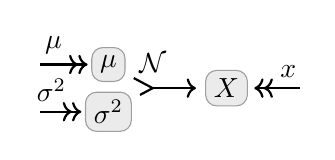
\begin{tikzpicture}[center base]
			\node[dpad0](X) at (0,0){$X$};
			% \node[dpad
			\draw[arr2, <<-] (X) to node[above,pos=0.7]{$x$} ++(1.0,0);
			% \draw[arr2, <-] (X) to node[above]{$\mathcal N(X|\mu,\sigma^2)$} ++(-1.7,0);
			\node[dpad0](m) at (-1.5, 0.3) {$\mu$};
			\node[dpad0](s2) at (-1.5, -0.3) {$\sigma^2$};
			\mergearr{m}{s2}{X};
			\node[above=2pt of center-ms2X](N){$\mathcal N$};
			\draw[arr1, <<-] (m) to node[above, pos=0.7]{$\mu$} +(-0.9,0);
			\draw[arr1, <<-] (s2) to node[above, pos=0.7]{$\sigma^2$} +(-0.9,0);
		\end{tikzpicture}}.
	\]

	The fisher information for a normal distribution is given by
	\[
	\mathcal I(\mu, \sigma) =
	% \begin{bmatrix}
	%     \Ex_{\mathcal N(X|\mu,\sigma^2}[ \frac{\partial mathcal N(X|\mu,\sigma^2}{\partial \mu}) ]
	% \end{bmatrix}
	% =
	\begin{bmatrix}
		\frac1{\sigma^2} & 0 \\
		0 & \frac{1}{2 \sigma^4}
	\end{bmatrix}
	\]



	The natural gradient update rule is given by
	\[
		F'_{x}(\mu, \sigma^2) = - \hat\nabla_{\mu, \sigma^2} \mathcal L(x,\mu,\sigma^2) = \mathcal I(\mu, \sigma^2)^{-1}
		\begin{bmatrix}
			\frac{x-\mu}{\sigma} \\[1ex] \frac {-\sigma^2 + (x-\mu)^2}{2 \sigma^4}
		\end{bmatrix}
		=
		\begin{bmatrix}
			x-\mu \\ (x-\mu)^2 - \sigma^2
		\end{bmatrix}
	\]

	Note that:
	\begin{itemize}
		\item  $\Ex_{x \sim \nu} [ F'_x(\mu,\sigma^2) ] = \mat 0$ if and only if $\nu$ has mean $\mu$ and variance $\sigma^2$.
		% We can interpret this in two ways:
		% This means that if observations are drawn from a fixed distribution $\nu(X)$,
		Moreover, this point is the unique global attractor.
		This means that,
		\begin{enumerate}
			\item If observations are drawn from a fixed distribution $\nu(X)$, and we repeatedly use $F$ to update $\theta = (\nu, \sigma)$ with small confidence $\epsilon$,
			then $\mu$ will approach the mean $\Ex_{\nu}[X]$ of $\nu$
			and $\sigma^2$ will approach the variance $\Ex_{\nu}[X^2] - \Ex_{\nu}[X]^2$.
			% If we make f observations are drawn from a fixed distribution $\nu(X)$,
			% If we update our belief parameters $\theta = (\mu, \sigma)$ according to $F$ with

			\item If we perform a single high-confidence update on the extended observation $\varphi \propto \nu$, in which each $x$ has relative confidence $\nu(x)$, the result will be a Gaussian with the mean and variance of $\nu$, i.e.,
			\[
				\forall \theta.\quad
				\lim_{c \to \infty} \Pr\nolimits_{F_{\nu}^c(\theta)} = \mathcal N(\Ex\nolimits_{\nu}[X], {\mathrm{Var}}_{\nu}[X])
			\]
		\end{enumerate}
		In this sense, relative confidence acts like probability.
		% So,

		\item
		If we update with the observation $x = \mu$ of our estimate with confidence $c$,
		the mean is unchanged, and our estimate of the variance becomes the harmonic mean of our previous variance $\sigma_0^2$ and the inverse confidence $\frac1c$.
		That is,
		\[
			F^c_\mu(\mu, \sigma_0^2) =
			\left(\mu, \frac{1}{c + \frac{1}{\sigma_0^2}} \right).
		\]
		In particular, if $\sigma_0^2$ is very large, so that our initial beliefs say very little, updating with confidence $c$ results in variance $\frac1t$.
		In this sense, the magnitude of confidence acts as the inverse of variance.
	\end{itemize}
\end{examplex}


%
\section{Internal Confidence}
a
% We now study how one constructs a belief state from a confidence measure.
Fix a set $\Phi$ of assertions.
We now study a natural way of constructing a space of beliefs $\Theta$ and a \cofunc $F$ for it,
which might be summarized as an internal log of changes in confidence. 


First, suppose $\Phi$ is a finite set $\{ \phi_1, \ldots \phi_n\}$, and $\confdom = \Rplus$. 
Then, define
\begin{align*}
	\Theta := \confdom_{\mathit{fin}}^{\Phi} := 
		\Big\{ \text{vectors}~ v \in \mathbb R^n \Big\}
\end{align*}
where 
$\confdom_{\mathit{fin}}^\Phi$ is the space of functions from $\Theta$ to $\confdom$ that map only finitely many elements of $\Phi$ to $\bot$.


% We now study a natural way of constructing a space of beliefs $\Theta$ and an update function, from a space $\Phi$ of assertions. 
% In a deep sense, this is a universal construction.





In fancier mathematical language, the material of this section may be seen as studying the final coalgebras of the signature 
$
	G := (-)^{\Phi \times \confdom} \times B
$
modulo the co-equations \cref{ax:certainty,ax:zero} in the category of manifolds and differentiable maps.


\begin{prop}
	The final coalgebra for the signature $G(-) = (-)^{\Phi \times \confdom}$
\end{prop}


\section{Settings}
\subsection{Probabilities and Samples}

First, let's take the where belief state is an explicit representation of a finite probability distribution, and observations are samples of it. 
Concretely, this means $\Theta := \Delta W$, and $\Phi := W$. 

% Intuitively, we would like it to be the case, that if we observe samples drawn from our 
Now, if observations are drawn from some true distribution $\mu^*$, then we would hope that 

\begin{CFaxioms}
	\item  $\bar F_{\!\mu}'\mu = \vec 0$. 
	That is, $\Ex_{x \sim \mu}[ F'_{\!x}\mu] = \vec 0$.
	\hfill \textbf{(sampling calibration)} \label{ax:sample-calibration}
\end{CFaxioms}

\begin{computation}
    Fix a ``transprot cost'' $c : W\times W \to \mathbb R$. 
    When is 
    \tcblower
\end{computation}


\begin{prop}
	Expected utility maximizing update rules cannot be calibrated for more than one distribution.

\end{prop}
\begin{lproof}
	Suppose we have a \cofunc\ given by
	$\mathcal L^{F}(\mu, x) = \Ex_{y \sim \mu} U(x,y)$.
	Then
	\[ 
		F'_{x} \mu = \mu \odot (\vec U_x - \Ex_{\mu}{U_x})
	\] 
	It is calibrated iff 
	\begin{align*}
		\vec 0 =  \bar F'_\mu(\mu) 
			&= \sum_{x} \mu(x)  F'_{x} (\mu)
			= \sum_{x} \mu(x) \Big( \vec \mu \odot \vec U_x - (\Ex\nolimits_{\mu}{U_x}) \vec \mu \Big) \\
		\iff\qquad
		\forall y \in X.~~
			0 &= \sum_{x} \mu(x) \mu(y) ( U(x,y) - \Ex\nolimits_{\mu} U_x ) \\
		\iff\qquad
		\forall y \in X.~~
			\Ex_{x \sim \mu}\Ex_{z\sim \mu}[ U(x,z) ] &= \Ex_{x \sim \mu}[ U(x,y) ]
	\end{align*} 
    
    \begin{phaseout}
	Choosing $\mu = \delta_w$, we this means
	\begin{align*}
		\forall y.~~ U(w,w) = U(w,y)
	\end{align*}
	but this means updating with respect to $x$ does nothing at all, no matter what state you're at.
	\TODO[\color{gray!50!red!50!white}TODO: this can be done without leaning so hard on degenerate distributions?]
    \end{phaseout}
    
    In particular, for $U(x,y) = \mathbbm 1[x=y]$, this means 
    \[
        \forall y \in X.~~
        \Ex_{x \sim \mu}\mu(X=x) = \mu(X=y),
    \]
    so $\mu(X=y)$ is the same for all $y$, meaning that $\mu$ is uniform.
    Therefore, $\mathit{Bolz-}\mathbf{1}$ is only calibrated for the uniform distribution.
\end{lproof}


\begin{prop}
    With respect to the Fisher metric, the loss function generating the linear combination \cofunc\ 
    \[
        \mathit{LIN}^c_{x}(\mu) = (1-c) \mu + c \delta_x
    \]
    is log loss
    $
        % F'_x (\mu) = 
        \mathcal L(\mu, x) = \log \mu(x) 
    $
\end{prop}
\begin{proof}
    \begin{align*}
    - F'_x = \hat \nabla_{\mu} \log \mu(x) &=  
        % \mu \odot \frac{1}{\mu} 
        \mathcal I(\mu)^{-1} \nabla_\mu \log \mu(x) \\
        &= \mu \odot \left(\Big[ \cdots, \frac1{\mu(x)}\frac{\partial}{\partial \mu_i} \mu(x), \cdots \Big] - \lambda \vec 1 \right) \\
        &= \Big[\cdots, \mathbbm1[x=i] - \lambda \mu(i) ,\cdots\Big] \\
        &= \delta_x - \mu            
    \end{align*}
    Note, that
    \begin{align*}
        \mathit{LIN}'_x = \frac{\partial}{\partial c} \mathit{LIN}^c_x(\mu) \Big|_{c=0} 
            = \frac{\partial}{\partial c} \Big[ (1-c) \mu + c \delta_x \Big]_{c=0} = \delta_x - \mu
    \end{align*}
    which is the same vector field.  
\end{proof}

Note that the value of the extended loss is cross entropy:
\begin{align*}
    \mathcal L^{\overline{\mathit{LIN}}}(\mu, \nu) = \Ex_{\nu} \log(\mu)
\end{align*}

% \begin{prop}
% The update rule given by 
% $
%     % F'_x (\mu) = 
%     \mathcal L(\mu, x) = \log \mu(x) 
% $
% is sample-calibrated.
% \end{prop}
% and this \cofunc\ is sample-calibrated.
\begin{prop}
    LIN is sample-calibrated.
\end{prop}
\begin{proof}
    $ \bar F'_\nu(\mu) = \Ex_{x \sim \nu}[ \delta_x - \mu ] = \nu - \mu$ 
    which is zero if and only if $\mu = \nu$.
\end{proof}


\begin{conj}
    Every sample-calibrated \cofunc\  is also quasi-linear. 
\end{conj}
\begin{conj}
    LIN is the only sample-calibrated \cofunc\ that satisfies
    \cref{ax:zero,ax:diffble,ax:effectiveness}.
\end{conj}

\subsection{Probabilities and Events}
Now, we consider the setting where $\Theta = \Delta W$ and $\Phi = 2^W$. 


Here are some update rules:
% \begin{table}
\begin{center}
\def\arraystretch{1.5}
\begin{tabular}{c|ccc|c}\toprule
    Dynamics $F$ & Flow $F^c_A(\mu)$
        & Vector Field $F'_A(\mu)$
        & Loss $\mathcal L^{F}(\mu, A)$
        & $F^c_A, F^{d}_B$ commute?
        \\\midrule
    $\mathit{LIN}$
        & $%\mathit{LIN}^c_A \mu =
            (1-c)\,\mu + (c)\,\mu| A$
        & $%\mathit{LIN}'_A \mu = 
            \mu| A - \mu$
        & $%\mathcal L^{\mathit{LIN}}(\mu, A) = 
            - \log \mu(A)$
        & if $\mu(A \cap B) > 0$ 
        \\[0.5ex]  %\noalign{\smallskip}
    $\mathit{LLI}$
        & {\def\arraystretch{0.8}
            \begin{tabular}{@{}l@{}}
            $\propto
                \mu^{1-c}\, (\mu|A)^c$\\
                \color{gray}
            $\propto
                \mu\, \mathbbm1_{A}$
            \end{tabular}}
        & {\color{red} N/A }
        & {\color{red} N/A }
        & always\\[1.5ex] %\noalign{\smallskip}
    $\mathit{Bolz}[\mathbf 1]$
        & {\def\arraystretch{0.9}\begin{tabular}{@{}l@{}}
            $\propto
                \mu \cdot \exp( \beta \mathbbm{1}_A)$\\
            \color{gray}
            $\propto
                \mu \cdot \exp( - \beta \mathbbm{1}_{\bar A})$
            \end{tabular}}
        & $\mu \odot (\mathbbm{1}_A - \mu(A))$ 
        & $\mu(\lnot A)$
        & always \\
    \bottomrule
\end{tabular}
\end{center}

Suppose $m$ is a distribution over events with $m(\emptyset) = 0$.
Let $\Pr_m$ be the distribution over $W$ given by
\begin{align*} 
    \Pr_m := \sum_{\substack{\emptyset \ne A \in \Phi}}
        m(\phi) \mathrm{Unif}_A 
    \qquad\qquad
    = B \mapsto
    % \Pr_m(B) :=
        % \sum_{A : A \cap B \ne \emptyset} 
        % \sum_{A \ne \emptyset} 
        \sum_{\emptyset \ne A \in \Phi} 
        % \sum_{A} 
        m(A) \frac{|B \cap A|}{|A|}.
\end{align*}
where $| - | : 2^W \to \mathbb R^{\ge 0}$ is a base measure on $W$, such as the counting measure when $W$ is finite.
A sanity check: this is indeed a distribution, since
$
    \sum_{A \ne \emptyset} m(A) \frac{|A|}{|A|} = \sum_{A \ne \emptyset} m(A) = 1
$.

In the language of graphical models, $\Pr_m$ is the distribution over $W$ given by the composite  
\[
    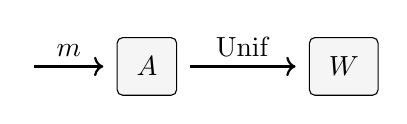
\begin{tikzpicture}
        \node[dpadded] (A) at (0,0) {$A$};
        \node[dpadded] (W) at (2.5,0) {$W$};
        
        \draw[arr2, <-] (A) to node[above]{$m$} ++(-1.5, 0);
        \draw[arr2] (A) to node[above]{$\mathrm{Unif}$} (W);
    \end{tikzpicture}
\] 

\begin{defn}
    % A \cofunc\ F is 
    % \emph{sample-calibrated} at $m$ 
    % if 
    % $
    %     \bar F'_{m}(\Pr\nolimits_m) = \vec 0.
    % $ 
    A \cofunc\ F is 
    $m$-\emph{sample-stationary} at $\mu$ 
    if 
    $
        \bar F'_{m}(\mu) = \vec 0.
    $ 
    % if $|| \bar F'_m( \Pr\nolimits_m) ||$ 
\end{defn}

\begin{computation}
    
% \begin{conj}
%     % \[
%     % F^\beta_A(\mu) = 
%     % \]
    $\mathit{LIN}$
    is $m$-sample-stationary at $\mu$ iff $\cdots$
    \tcblower
% \end{conj}
% \begin{proof}
    $\mu$ is a fixed point of samples drawn from $m$ iff
    \begin{align*}
        \forall x.~
        0 = \sum_{A \ne \emptyset} m(A) (\mu(x|A) - \mu(x)) 
        = \sum_{A \ne \emptyset} m(A) \left(
            \frac{\mu(x) \mathbbm1[x \in A]}{\mu(A)} - \mu(x) \right) \\
        = \mu(x) \sum_{A \ne \emptyset} m(A) \left(
            \frac{\mathbbm1[x \in A]}{\mu(A)} - 1 \right) \\
    \end{align*}
    which means, for every $x$ with $\mu(x) > 0$, we have
    \begin{align*}
        0 &= \sum_{A \ne \emptyset} m(A) \left( \frac{\mathbbm1[x \in A]}{\mu(A)} - 1 \right)  \\
          &= \sum_{A \ne \emptyset} m(A)\frac{\mathbbm1[x \in A]}{\mu(A)} - \sum_{A \ne \emptyset}m(A) \\
          \iff\qquad
          1 &=  \sum_{A \ni x}\frac{m(A)}{\mu(A)} \\
        % \iff\qquad  0 = \sum_{A \ne \emptyset} m(A) \left( \frac{\mathbbm1[x \in A]}{\mu(A)} - 1 \right)
    \end{align*}
    % Observe that this quantity is strictly larger than 
    Obviously if $m = \delta_W$, then this will be the case, and after all, conditioning on the trivial event does nothing, and results in the trivial vector field. 
    
    What about for others? Clearly if $m = \delta_{\{x\}}$, this is true iff $\mu = \delta_x$, which is also appropriate.
    
    What about other point masses? If $m = \delta_B$, for some set $B$, then the condition states that $\mu(B) = 1$, which also seems reasonable.
    
    Now, what if $m$ corresponds to a probability distribution? Our condition becomes
    \[
        \forall x.~ \sum_{\{y\} \ni x} \frac{m(\{y\})}{\mu(y)} = \frac{m(\{x\})}{\mu(\{x\})} = 1
    \]
    which is to say that $\mu$ is equal to the distribution that $m$ corresponds to.
    
    
    Great. Now suppose that $m = s \delta_B + (1-s) \delta_W$ is a simple support function for $W$.  The condition becomes
    \[
        \forall x \in B.~ 1= \frac{s}{\mu(B)} + \frac{1-s}{1} 
        \qquad\iff\quad
            \mu(B) = s + \mu(B) - s \mu(B)
        \quad\iff\quad
            0 = s (1 - \mu(B))
    \] 
    so, supposing $s > 0$, once again, this is only stationary if $\mu(B) = 1$. Of course, this isn't too surprising either, since it's also a concentric mass function.
    
    More generally, let's take $m = (s)\delta_A + (1-s)\delta_B$, and suppose $A \ne B$.
    Now, $\mu$ is stationary iff
    \begin{enumerate}
        \item If $A \cap B \ne \emptyset$, then
        $\displaystyle 
            \frac{s}{\mu(A)} +  \frac{1-s}{\mu(B)} = 1
        %    
        $
        % \begin{align*}
        %     \iff\quad s\,\mu(B) + (1-s)\,\mu(A) = \mu(A) \mu(B) \\
        %     \iff\quad s\,\mu(B) - s\,\mu(A) = \mu(A) (\mu(B) - 1) \\
        %     \iff\quad s = \frac{\mu(A) \mu(B) - \mu(A)}{\mu(B) - \mu(A)} 
        %         = \frac{\mu(B) - 1}{\frac{\mu(B)}{\mu(A)} - 1}
        %         % = \frac{1 - \frac{1}{\mu(B)}}{\frac{1}{\mu(A)} - \frac{1}{\mu(B)}}
        %         % = \frac
        %         % \\
        % \end{align*}
        which is to say the weighted harmonic mean of $\mu(A)$ and $\mu(B)$ is one; since the harmonic mean lies between the minimum and maximum values, and since probability is at most 1, this means we must have $\mu(A) = \mu(B) = 1$.
        
        \item If $\exists x \in A \setminus B$ with $\mu(x) > 0$ then 
        $\displaystyle
            \frac{s}{\mu(A)} = 1 \quad \iff\quad \mu(A) = s > 0;
        $

        \item If $\exists x \in B \setminus A$ with $\mu(x) >0$, then 
        $\displaystyle
            \frac{1-s}{\mu(B)} = 1 \quad \iff\quad \mu(B) = 1-s >0;
        $
    \end{enumerate}
    % Taken together, (1) and (2) imply that if $\mu(A \setminus B) > 0$ and $\mu(A \cap B) > 0$ then
    % \[ \mu(A) (\mu(B) - \mu(A)) = \mu(A) (\mu(B) -1) \quad\iff\quad
    %     \mu(A) = 1 \]
    % and symmetrically, if $\mu(B \setminus A) > 0$ and $mu(A \cap B) > 0$, then
    Since $A \ne B$, either (2) or (3) must hold, and so if $A$ and $B$ are not disjoint, then there are no stable points that puts mass outside of $A \cap B$. 
        
    On the other hand, if $A$ and $B$ are disjoint, we have shown that the stable distributions are the ones that have $\mu(A) = s$  and $\mu(B) = 1-s$.  
    
    
    % What if $m = \frac13\delta_{\{a,b\}} + \frac13\delta_{\{b,c\}} + \frac13\delta_{\{c,a\}}$
    What if $m = m_{\bar c}\delta_{\{a,b\}} + m_{\bar a}\delta_{\{b,c\}} + m_{\bar b}\delta_{\{c,a\}}$
    % By symmetry, we expect that the only fixed point is the uniform distribution over $\{a,b,c\}$. 
    Suppose that there is a fixed point $\mu$ with all positive probabilities. Then,
    \begin{align*}
         1 = \frac{m(\{a,b\})}{\mu(a) + \mu(b)} + \frac{m(\{a,c\})}{\mu(a) + \mu(c)} 
         = \frac{m(\{a,b\})}{\mu(a) + \mu(b)} + \frac{m(\{b,c\})}{\mu(b) + \mu(c)} \\
         \Rightarrow \qquad
         \frac{m(\{a,c\})}{\mu(a) + \mu(c)} = \frac{m(\{b,c\})}{\mu(b) + \mu(c)} = \frac{m(\{a,b\})}{\mu(a) + \mu(b)} =: k.
    \end{align*}
    So $\mu(\{a,b\}) + \mu(\{b,c\}) + \mu(\{a,c\}) = 2 = \frac{1}{k}m(\{a,c\}) + \frac1km(\{b,c\}) + \frac1k m(\{a,c\})$. So $k=\frac12$. Thus we can solve
    \begin{align*}
        \begin{bmatrix}
            1 & 1 & 0 \\
            1 & 0 & 1 \\
            0 & 1 & 1
        \end{bmatrix}
        \begin{bmatrix}
            \mu(a) \\ \mu(b) \\\mu(c)
        \end{bmatrix}
        &= 
        \frac1k
        \begin{bmatrix}
            m(\{a,b\}) \\ m(\{a,c\}) \\ m(\{b,c\})
        \end{bmatrix}\\
    \qquad\implies\qquad& 
        \mu = 2
            \begin{bmatrix}
                1 & 1 & 0 \\
                1 & 0 & 1 \\
                0 & 1 & 1
            \end{bmatrix}^{-1}
            \begin{bmatrix}
                m(\{a,b\}) \\ m(\{a,c\}) \\ m(\{b,c\})
            \end{bmatrix}
        = 
        \begin{bmatrix}
            1 & 1 & -1 \\
            1 & -1 & 1 \\
            -1 & 1 & 1
        \end{bmatrix}
        \begin{bmatrix}
            m(\{a,b\}) \\ m(\{a,c\}) \\ m(\{b,c\})
        \end{bmatrix}
    \end{align*}
    Since probability must be non-negative, we also find that there is only a fixed point
    with positive probability on all events if each mass is less than the sum of the other two. 
    Otherwise, say $m(\{a,b\}) > \frac12$ --- there is not enough support for $c$ even split between $\{b,c\}$ and $\{a,c\}$ to overcome the evidence in favor of $\{a,b\}$, and so any positive probability on $c$ must shrink to zero.
        
    % Now, if $\mu = \Pr_m$, then $\mu(A) = \sum_{\emptyset \ne U  \in \Phi} m(U) \frac{|U \cap A|}{|U|}$, so our condition becomes
    % \begin{align*}
    %       1 &=  \sum_{x \in A \ne \emptyset}\frac{m(A)}{\sum_{\emptyset \ne U  \in \Phi} m(U) \frac{|U \cap A|}{|U|}} \\
    % \end{align*}
% \end{proof}


\begin{conj}
    If $\mu$ is a fixed point of $\mathit{LIN}_m$, then 
    $\mu(A) \ge \mathrm{Bel}_m(A)$ for all events $A$.
    \\
    That is, $\mathrm{Fixedpts}( \mathit{LIN}_m ) \subset \mathcal P_m$.
\end{conj}
\begin{proof}
    Suppose $\mu$ is a fixed point of $\mathit{LIN}_m$.
     % and let $S := \{ x : \mu(x) > 0\}$.
    First we show that if $\mu(A) = 0$, then $m(A) = 0$. 
    
    \TODO[THIS IS FALSE --- see example above. Proposition cannot be proved this way.]
    
    % If $\mu(A) = 0$, then $\mu(x) = 0$ for all $x \in A$.  
    % Suppose $\mu(A) = 0$.
    % Any set $B$ containing a point $y$ with positive probability must not be a subset of $A$.  
    % % The fixed point condition above then says that for some $y : \mu(y) > 0$,
    % \[
    %     % 1 = \sum_{B \ni y} \frac{m(B)}{\mu(B)} \le \sum_{B : B \not \subset A} \frac{m(B)}{\mu(B)}
    %     1 = \sum_{B : \mu(B) > 0} \frac{m(B)}{\mu(B)}
    % \]
    % and the summation does not contain any subsets of $A$. 

    

    By the computation above, we know that
    \[ 
        \sum_{B : \mu(B) > 0} \frac{m(B)}{\mu(B)} = 1
    \]
    Then if $A$ is an event with $\mu(A) > 0$,
    \begin{align*}
        \mu(A) &= m(A) + \sum_{B \ne A: \mu(B) > 0} \frac{m(B) \mu(A)}{\mu(B)} \\
        &\ge m(A) + \sum_{B \subsetneq A: \mu(B) > 0} \frac{m(B) \mu(A)}{\mu(B)} 
            &\text{since this is only a subset of the terms}\\
        &\ge m(A) + \sum_{B \subsetneq A: \mu(B) > 0} m(B)
            &\text{since $\mu(A) \ge \mu(B)$ when $A \supset B$} \\
        &= \sum_{B \subset A;\,\mu(B)>0} m(B)  \\
        &= \mathrm{Bel}_m(A) - \sum_{B \subset A : \mu(B) = 0} m(B).
    \end{align*}
    
\end{proof}
We know that the converse does not hold, because if the intersection of all sets $A$ with $m(A) > 0$ is non-empty, then any fixed point must be supported entirely on $A$ --- and yet, if $m(W) > 0$, then there are probability distributions in $\mathcal P_m$ that have full support, including $\Pr_m$. 

 
\end{computation}

% \end{table}


\subsection{Probabilities and Probabilities}

% \begin{enumerate}
%     \item 
% \end{enumerate}
First, full, unconditional distributions. 
\begin{center}
\begin{tabular}{c|ccc|c}\toprule
    Dynamics $F$ & Flow $F^c_q(\mu)$
        & Vector Field $F'_q(\mu)$
        & Loss $\mathcal L^{F}(\mu, q)$
        & Properties
        \\\midrule
    $\mathit{LIN}$
        & $%\mathit{LIN}^c_A \mu =
            (1-c)\,\mu + (c)\, q$
        & $%\mathit{LIN}'_A \mu = 
            q - \mu$
        & $%\mathcal L^{\mathit{LIN}}(\mu, A) = 
            \kldiv{q}{\mu}$
        & \\ 
    $\mathit{LLI}$
        & $\propto
            \mu^{1-c}\, q^c$
        & $\mu \odot \Big( \log \frac\mu q - \kldiv\mu q \Big)$ 
        & $\kldiv\mu q$ 
        &\\
    \bottomrule
\end{tabular}
\end{center}

If $F$ is an update rule for $W$, then $\bar F$ is an update rule for $\Delta W$. 
% Thus, every 

There are also analogous update rules when observations are not full joint distributions, but rather only conditional marginals of them.



\section{Examples}
\subsection{Assorted}

\begin{examplex}{Internal Confidence}{}
	C
\end{examplex}

\subsection{Relaxations of Bayes Rule (Updating By Conditioning)}
Fix some measurable space $\X = (X, \mathcal A)$ of possible outcomes, and consider an update rule for probability distributions $\Theta := \Delta\X$
on measurable events $\Phi = \mathcal A$.

The function
\[
	\mathrm{Bayes}^\beta_A(\mu) := \begin{cases}
			\mu \mid A &  \text{if }\beta > 0 \\
			\mu & \text{if } \beta = 0 \\
			\mu \mid \bar A &  \text{if } \beta < 0
		\end{cases}
\]
satisfies \cref{ax:zero,ax:additivity}, so it is an update rule.  But it is not differentiable in $\beta$ (it doesn't satisfy \cref{ax:diffble}).
% owever, it can be written as a limit of one that does:
% However, this behavior does arise as the limit of large $\beta$ for a differentiable update rule:
However, this behavior does arise as the limit of large-magnitude $\beta$ for a differentiable update rule. Consider the update rule
\begin{align*}
	F^\beta_A (\mu) &:\propto \mu \exp(\beta \mathbbm1[A]) \\
	F^\beta_A (\mu)(B) &:=
		% \mu(B) \exp(\beta \mathbbm1[A \cap B])
		\frac{1}{\Ex_{\mu}[e^{\beta\mathbbm1[A]}]}\int_{X}  \mathbbm1[B] \exp(\beta \mathbbm1[A]) \mathrm d\mu \\
		&=
		\frac{\mu(B\cap A)e^{\beta} + \mu(B \cap \bar A) }
		% {\mu(A)e^{\beta} + (1 - \mu(A))}
		{\mu(A)e^{\beta} + \mu(\bar A)}.
		% \int_{X}  \mathbbm1[B] \exp(\beta \mathbbm1[A]) \mathrm d\mu
\end{align*}

% It is easy to check that $F$ satisfies
% \cref{ax:zero,ax:additivity,ax:certainty,ax:symmetry,ax:commute,ax:diffble,ax:invert}.
% In addition to being a flow, this update rule
Note that
\begin{align*}
\lim_{\beta\to\infty} F^\beta_A(\mu) &= B \mapsto \frac{\mu(B \cap A)}{\mu(A)}
   = \mu \mid A; \\
 F^0_A(\mu) &= B \mapsto \mu(B); \qquad\text{and}\\
\lim_{\beta\to-\infty} F^\beta_A(\mu) &= B \mapsto \frac{\mu(B \cap \bar A)}{\mu(\bar A)}
	  = \mu \mid \bar A.
\end{align*}
Thus, $\mathrm{Bayes} = \lim_{k \to \infty} F^{k}$, where $F^k$ is the update rule given by rescaling, as in \cref{prop:rescale}.



\begin{wip}
Is this the only such relaxation of Bayes Rule?

Suppose $F$ is another such relaxation, satisfying \cref{ax:zero,ax:additivity,ax:certainty,ax:symmetry,ax:commute,ax:diffble,ax:invert}.

\begin{prop}
	$F$ is unique up to curve reparameterization.
\end{prop}

By differentiability (\cref{ax:diffble}) and \cref{thm:vecrep}, we know that $F$ is generated by vector field $F' : \mathcal A \times \Delta\X \to \Delta\X$.
We start by investigating the action on singletons.
\[
	F'_{\{x\}}(\mu)
\]

Assuming that the vector field is conservative,

\begin{conj}
	$F$ is the unique update rule, up to multiplicative scaling, satisfying
	\cref{ax:zero,ax:additivity,ax:certainty,ax:symmetry,ax:commute,ax:diffble,ax:invert}
\end{conj}
\end{wip}


% \subsection{Case Study: Jeffrey's Rule}
\subsection{Confidence as a Belief State: Mixture of Experts}

\subsection{Weight of Evidence}
\subsection{Loss Functions}
\subsection{Calibration}

Suppose $Y$ is a finite set $\{y_1, \ldots, y_m\}$, and
a classifier $p : \Theta \times X \to \Delta Y$, which for a parameter setting $\theta \in \Theta$, yields a predictor $p_\theta Y$. 
In practice, this is typically implemented by taking applying a `softmax layer' to final layer of a neural network (with weight space $\Theta$). 
Concretely, suppose $\lambda(Y)$ is a base measure on $Y$, and the output of the final layer of the network (for fixed weights $\theta$ and input $x$) is a vector $\mat v\in \mathbb R^{m}$. 
Then $p_\theta(Y=y_i|x) := \sigma_k(\mat v) := \lambda(y_i) \exp(\beta \mat v_i) / \sum_j \lambda(y_j) \exp(\beta v_j)$. 
where $\beta \ge 0$ is sometimes known as the ``inverse temperature'' of the softmax, and is typically fixed at $\beta=1$. 

% Now, suppose you have an output $\mat v$. Ho
% Now, this inverse temperature can 
This inverse temperature can be viewed as a measure of confidence. 
At one extreme, when $\beta = 0$, $p_\theta(Y|X) = \lambda(Y)$, corresopnds to having ``no confidence in the network'', in the sense that we ignore its predictions and output our ``prior belief'' $\lambda(Y)$. 
At the opposite extreme, when $\beta = \infty$, the output distribution will be a point mass on the value $y_j$ for which $\mat v_j$ is maximal.
This indicates ``full confidence'', in the sense that 

This also corresponds to 

In the presence of a ``true'' emperical distribution $\mu(X,Y)$, such a classifier is called ``calibrated'' if $p_\theta(Y|X) = \mu(Y|X)$. 

\subsection{Bolzman Rationality}

\begin{examplex}{}{}
	Consider a neural network whose output is a c
\end{examplex}

% Loss Functions
% Total \# of Updates
\section{Confidence in PDGs}
\subsection{Quantitative PDGs}

\subsubsection{Updating Second-Order Distributions with PDGs}
Let $\N$ be a set of variables, where each variable $X \in \N$ can take possible values in the set $\V(X)$, and let $\V(\N)$ be the set of possible joint settings of all variables in $\N$.

\begin{align*}
	\Theta &:=
		\Big\{
		\text{Second-order probabilities}~ \Pr \in \Delta^2 \V(\N)
		\Big\} \\
	% \Phi &:= \Big\{ \text{PDGs}~ \dg M
	%     \text{ with variables } \N^{\dg M} = \mat X \Big\}
	\Phi &:= \Big\{ \text{cpds}~ p(Y|X)
		% \text{ where }  X, Y \in \mat X \Big\}
		\text{ where }  X, Y \subset \N \Big\}
		%%% TODO: What about hypergraph fs non-hypergraph distinction?
\end{align*}

Now, consider the Bolzmann update rule
% Given a PDG $\dg M$, let $\X := \Delta\V(\dg M) = \Delta(\prod_{X\in\N}\V(X))$. For each edge we have
\[
	F_L^{\beta}(\Pr) (\mu) \propto \Pr(\mu) \exp(-\beta \kldiv\mu \bp)
\]
which corresponds to the loss function
$\mathcal L^F(L, \Pr) = \Ex_{\mu \sim \Pr}[\kldiv\mu{\bp}]$.

% Note, that the free extension of $\Phi$ is
Note that the extended input space $\bar \Phi$ is isomorphic to the set of ``purely quantitative'' PDGs, i.e., those with $\balpha = \mat 0$, over the variables $\mat X$: $$
	% \bar\Phi = \{ \text{PDGs}~\dg M \text{ with variables } \N^{\dg M} = \mat X \Big\}
	\bar\Phi = \Big\{ \text{PDGs}~\dg M = (\mat X, \Ed, \bP[], \mat0, \bbeta) \Big\}
$$
and it is easily verified that update rule from before extends to
\[
	F_{\dg M}^k(\Pr)(\mu) \propto \Pr(\mu) \exp(- k \bbr{\dg M}_0(\mu))
\]
Note that
\begin{align*}
	\lim_{k \to \infty} F_{\dg M}^k(\Pr)(\mu) &\propto
		% \mathbbm1[\mu \in {\displaystyle\SD{\dg M}}]
		\Pr(\mu) \mathbbm1[\mu \in {\bbr{\dg M}^*_0}] \\
		&= \Pr \,|\, \bbr{\dg M}^*_0 \\
		&= \Pr \,|\, \SD{\dg M} \text{~if $\dg M$ is consistent.}
		% &= \mathrm{Unif}_{\{\!\!\{{\dg M}\}\!\!\}} \text{~if $\dg M$ is consistent.}
\end{align*}

That is to say, applying the update with observation $\dg M$ and infinite certainty is like conditioning the higher-order distribution $\Pr$ on those distributions $\mu$ consistent with $\dg M$.
% On the other hand,
Now we turn to the opposite extreme, when confidence is low. When $k=0$, clearly $F^k_\dg M(\Pr) = \Pr$, so $F$ satisfies \cref{ax:zero}. And in the limit,
% as $\gamma \to 0$,
\begin{align*}
	\lim_{k \to 0} F_{\dg M}^k(\Pr)(\mu) &= \Pr \,|\, \{ \Inc_{\dg M}(\mu) < \infty \} \\
		&= \Pr \,|\, \{\mu : \forall L.~\mu(Y|X) \ll \bp \}.
		% \quad\Big(\text{i.e., if $\mu$ is absolutely continuous with respect to $\bp$}
		% \Big)
\end{align*}

So $F$ can only be continuous at $k=0$ for $\Pr$ (and hence can only satisfy \cref{ax:diffble}) if, for all edges $L \in \Ed$, we have that $\Pr(\mu(Y|X) \ll \bp) = 1$.
One sufficient condition to ensure diefferentiablility (\cref{ax:diffble}) is to restrict to observations of strictly positive cpds.


\subsubsection{Updating Distributions with PDGs and Incompatibility}
% \def\tauur{\mathtt T}
% \def\tauur{\mathtt{GD}}
% \def\tauur{\tau}
\def\tauur{\mathtt{CPD\_UR}}

\begin{align*}
	\Theta &:=
		\Big\{
		\text{Joint probabilities}~ \mu \in \Delta \V(\N)
		\Big\} \\
	\Phi &:= \Big\{ \text{cpds}~ p(Y|X)
		% \text{ where }  X, Y \in \mat X \Big\}
		\text{ where }  X, Y \subset \N \Big\}
\end{align*}

Given a cpd $p(Y|X)$ with $X,Y \subset \mat X$,
define an update rule on joint distributions $\mu$ by
\begin{align*}
	% (\tau_{p(Y|X)}^\beta \mu) (\mat X) \propto
	%     \mu(X) \left(\frac{p(Y|X)}{\mu(Y|X)}\right)^{1 - e^{-\beta}} \mu(\mat X\setminus\{X,Y\}\mid X,Y)
	\Big(\tauur_{p(Y|X)}^\beta \mu\Big) (\mat X) &\propto
		\mu(\mat X) \left(\frac{p(Y|X)}{\mu(Y|X)}\right)^{1 - e^{-\beta}}
\end{align*}
	%
	% \\
	% &= \mu(X) p(Y|X)^{e^{-\beta}} \mu(Y|X)^{1-e^{-\beta}}  \mu(\mat X\setminus\{X,Y\}\mid X,Y)
%     &= \mu(X)\; p(Y|X)^{\epsilon} \mu(Y|X)^{1-\epsilon}  \mu(Z\mid X,Y)
% \end{align*}
Writing this in a
where $\epsilon := 1-e^{-\beta}$ and $Z := \mat X \setminus \{X,Y\}$.

\begin{prop}
	$\tauur_{p(Y|X)}$
\end{prop}

\begin{prop}
	The vector field of $\ext\tauur$ is the natural gradient of $\Inc_{\dg M}$, i.e.,
	$
		% \tau'_{\dg M}(\mu) = - \hat \nabla_\mu \bbr{\dg M}_0(\mu),
		\ext\tauur'_{\dg M} = - \hat \nabla \Inc_{\dg M},
	$
	so $\tauur$ is the update rule on joint distributions which reduces incompatibility by locally moving in the direction of steepest descent.
\end{prop}

\begin{prop}
	% \begin{enumerate}
		% \item \relax \texttt{\color{red}[CONJECTURE]}~
		% $\displaystyle
		%     \tauur_{\dg M}^{\{\nf1\gamma\}}(\mathrm{Unif}) \in \bbr{\dg M}_{\gamma}^*
		% $
		%
		% \item
		Updating $\dg M$ with absolute certainty computes the information projection onto the convex set of distributions consistent $\dg M$ i.e.,
		$$\displaystyle
			\tauur_{\dg M}^\infty(\mu) = \argmin_{\mu' \in \SD*{\dg M}} \kldiv{\mu'}{\mu}
		$$

	% \end{enumerate}
\end{prop}


\subsubsection{Updating PDGs with PDGs, via inconsistency reduction}
\begin{align*}
	\Theta :=
		\Big\{
		\text{PDGs}
		\Big\}; \qquad
	\Phi := \Big\{ \text{PDGs} \Big\}
\end{align*}

% Of course, we often think
We now consider the more general setting, in which both the observations $\Phi$ and the belief states $\Theta$ are
Here's an update rule that simply adds the new data to a PDG.
\[
	F^{\beta}_{p(Y|X)}(\dg M) = \dg M ~+~
		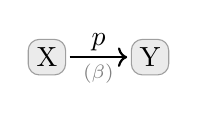
\begin{tikzpicture}[center base]
			\node[dpad0](X) {X};
			\node[dpad0,right=0.8 of X](Y) {Y};
			\draw[arr1](X) to
				node[above,inner sep=2pt]{$p$}
				node[below,inner sep=2pt]{${\scriptstyle\color{gray}(\beta)}$} (Y);
		\end{tikzpicture}
\]

It's extension is the update rule that incorporates data of the new PDG to the old one, where all confidences in the new PDG are scaled by $k$.
\[
	% F^{\beta}_{\dg M'}(\dg M) = \dg M ~+~ \beta\,\dg M'
	\bar F^{k}_{\dg M'}(\dg M) = \dg M ~+~ k\,\dg M'
\]

% There are actually several natural
The colletion of all PDGs, even on a finite set of finite variables, does not naturally form a manifold of fixed finite dimension.
But if we restrict our attention to PDGs with a certain fixed structure, then it does.
But, per \parencite{richardson2022loss}, we already have a natural choice of a loss $\mathcal L = \aar{-} : \mathrm{PDG} \times \mathrm{PDG} \to \mathbb R$: the inconsistency of the joint PDG.

Still, there is more than one reasonable way to perform updates: we can adjust the internal confidences $\bbeta$ of our PDG, or its cpds $\mat p$.
% The first is closer to a mixture of experts approach, and the latter

\[
	\bar G'_{\dg M'}(\dg M) = - \hat\nabla_{\mat p} \aar{\dg M + \dg M'}
\]

\begin{openQ}
	How do $\bar F$ and $\bar G$ relate to one another?
\end{openQ}

\begin{conj}
	$\tauur$ should be a special case.
\end{conj}

\subsubsection{}
\begin{align*}
	\Theta :=
		\Big\{
		\text{PDGs over variables } \mat X
		\Big\}; \qquad
	% \Phi := \Big\{
	%     \text{Probabilities}~ \mu \in \Delta \V(\mat X)
	%     \Big\}
	\Phi := \Big\{
		\text{Probabilities}~ \mu \in \Delta \V(\mat X)
		\Big\}
\end{align*}


\section{Other Confidence Domains}

% \begin{phaseout}
To describe a degree of partial incorporation, we will need a domain of possible confidence values.
Mostly, we will stick to using real numbers, but it will clarify things to stay more general for now, so that we can see the properties we actually need. 
% Formally, we represent the possible degrees of confidence by a group
Formally, a \emph{confidence domain} is a tuple $(\confdom, \oplus, \bot, \top)$, 
where $(\confdom, \oplus, \bot)$ is a monoid with operation $\oplus$ and neutral element $\bot$, and $\top \in \confdom$ is an absorbing element---i.e., $\top \oplus c = \top$ for all $c \in \confdom$.
In terms of confidence, we interpret the components as follows:

\begin{itemize}%[]
	\item
	The elements of $\confdom$ are the possible degrees of confidence.

	\item
	The monoid operation $\oplus : \confdom \times \confdom \to \confdom$ describes how to combine two (independent) confidences in some statement, to obtain a new confidence in that statement.     

	\item The neutral element $\bot \in \confdom$ indicates ``no confidence'' in an observation.
		%
		% The fact that we want to ignore information we have no confidence in
		% gives corresponds to the group identity laws: that
	The monoid identity laws, which assert that
		$\bot \oplus c = c = c \oplus \bot$ for all $c \in \confdom$,
	reflect the intuition that we should ignore untrusted information in combining confidences.
		% in which case we should ignore the information at hand,
	\item The absorbing element $\top$ indicates ``full confidence''.
	The absorbtion property corresponds to the intuition that, definitive information that $\phi$ is true, when combined with other (perhaps less reliable) information that $\phi$ is true, is still definitive.
\end{itemize}
% \end{phaseout}

In this more general setting, the analogue of additivity (\cref{ax:additivity}) becomes:
\begin{CFaxioms}
	\item For all $c_1, c_2 \in \confdom$,~
		% $F^{c_1}_\phi \circ F^{c_2}_\phi = F^{c_1 \oplus c_2}_\phi$
		$F^{c_1}_\phi \circ F^{c_2}_\phi = F^{c_1 \oplus c_2}_\phi$
		% \hfill \textbf{(additivity)} \label{ax:additivity}
		\hfill \textbf{(combination)} \label{ax:additivity}
\end{CFaxioms}
\Cref{ax:additivity} looks like it could be problematic, but it simply states that \cofunc s respect the combination operation. 
If we fix an assertion $\phi$, then an update with confidence $c_1$ followed by an update with confidence $c_2$ is equivalent to an update with confidence $c_1 \oplus c_2$, which is, by definition, the result of comining confidences $c_1$ and $c_2$.
On its own, so long as we have the freedom to choose $\confdom$, \Cref{ax:additivity} has no teeth. 


\begin{prop} \label{prop:free-additivity}
	If $F: \confdom \to (\Phi \to (\Theta \to \Theta))$ satisfies \cref{ax:zero,ax:idemp}, then we can construct a new update
	% function for $\Theta$ on $\Phi$, that behaves in exactly the same way, but \emph{is} additive, but with the altered confidence domain
	function for $\Theta$ on $\Phi$, that behaves in exactly the same way, except that it is exteneded to a larger confidence domain, for which which it does satisfy \cref{ax:additivity}. 
\end{prop}
\begin{lproof}
Consider the new confidence domain
$$
	\confdom' := \Big\{ \text{ finite lists } [c_1, \ldots c_n]
		\text{ with each } c_i \in \confdom, 
		% \text{ such that } c_i \in \confdom \text{ for all } i = 1, \ldots, n 
		\quad
		% \text{list concatenation}~::,
		::,
		\quad
		[\,],
		\quad
		[\top]
		\,
	\Big\},
$$
whose group operation ``$::$'' is list concatenation, except that it collapses instances of $\top$, i.e., 
\[ 
	[c_1, \ldots c_n] :: [d_1, \ldots, d_m]
	 := \begin{cases}
		 % [\top] & \text{ if } c_i = \top \text{ for some $i$ or $d_j=\top$ for some $j$}\\
		 [\top] & \text{ if } \top \in \{c_1, \ldots, c_n,d_1, \ldots,d_m \} \\
		 [c_1, \ldots, c_{n}, d_1, \ldots, d_m] & \text{otherwise.}
 \end{cases}
\]
Concatenating the empty list $[\,]$ on either side has no effect,
by construction, for all $L \in \confdom'$, we have $[\top] :: L = [\top] = L :: [\top]$, 
and $::$ is clearly associative, so $\confdom'$ is also a confidence domain.

The new update rule for this confidence is given by:
	\[
		AF^{[c_1, \ldots, c_n]}_\phi (\theta)  :=
				(F^{c_n}_\phi \circ \cdots \circ F^{c_1}_\phi) (\theta).
	\]
$AF$ has the same behavior as $F$ on the elements that correspond to the original confidence domain, since
$
	AF^{[c]}_\phi(\theta) = F^c_\phi(\theta),
$
and it is additive by construction, since
\begin{align*}
AF^{[c_1, \ldots, c_n]}_\phi ( AF^{[d_1, \ldots, d_m]}_\phi (\theta) )
		&:=
			F^{d_m}_\phi \circ \cdots \circ F^{d_1}_\phi (
			F^{c_n}_\phi \circ \cdots \circ F^{c_1}_\phi (\theta))\\
		&= (F^{d_m}_\phi \circ \cdots \circ F^{d_1}_\phi \circ
		F^{c_n}_\phi \circ \cdots \circ F^{c_1}_\phi) (\theta) \\
		&= AF^{[c_1, \ldots, c_n, d_1, \ldots, d_m]}_\phi (\theta) \\
		&= AF^{[c_1, \ldots, c_n] :: [d_1, \ldots, d_m]}_\phi (\theta).
\end{align*}
\end{lproof}% We are primarily interested in the case where confidence can be measured as a real number,
For convenience of measurement, and so that we may better study confidence as a \emph{smooth} interpolation between ignoring and fully incorporation, we shall focus primarily on cases where confidence can be measured as a real number.
% We now define two confidence domains that are real numbers between 0 and 1.
We now consider two such confidence domains.

\begin{itemize}
	\item 
	% Another confidence domain we could consider 
	First, we consider the zero-one confidence domain
	\[
		\ZO := \Big(~ [0,1],
			% \quad a \star b := a b,
			\quad a \star b := 
					% 1- (1-a)(1-b) =
					a + b - ab,
			\quad 1,
			\quad 0 ~\Big),
	\]
	which uses the same numerical endpoints as probability;
	a value of zero represents no confidence, a value of one represents full confidence.
	For the purposes of updating, we may interpret a confidence of $a \in \ZO$ as the fration of the way between ignoring and fully incorporating information. 
	This motivates the definition of the operator $\star$.
	If you go $90\%$ of the way to fully incorporaing some information $\phi$, and then $50\%$ of the remaining way, then in total you have gone $90\% + 50\%(100\%-90\%) = 0.9 + 0.5 - (0.9)(0.5)$ of the way to fully incorporating $\phi$.    
	
	% In this domain
	% Clearly, 1 is neutral and 0 is absorbing element.\end{itemize}
	\item
	% First, we consider the monoid of positive extended real numbers under addition.
	We now introduce a second confidence domain based on the real numbers,
	which is mathematically cleaner, if
		% at first
		more difficult to interpret numerically in absolute terms.
	\[
		\Rplus := 
			\Big([0, \infty) \cup \{\infty\}, 
				\quad +,
				\quad 0,
				\quad \infty
				~\Big)
	\]
	
	% The use of addition as the combination operator means that independent measurements add, which in turn makes it 
	The use of addition as the combination operator makes it particularly natural to speak of linear combinations of inputs. 
	% Here are some examples. 
	This point is best illustrated by example.
	
	\begin{itemize}
		\item \textbf{Voting.}  
		Suppose the elements of $\Phi$ correspond to candidates in an election.
		In a sense, the number of votes a candidate recieves is a measure of how much confidence the electorate has in them---a candidate who recieves no votes is ignored, while a candidate who recieves all of the votes should be listened to exclusively.
		
		It's hard to say much  the raw number of votes a candidate recives in absolute terms, in part becasue it depends on the number of votes recieved by other candidates, and also how many votes you will recieve in the future. 
		% Nevertheless, it is still m
		Nevertheless, if we are collecting votes, is especially natural to weight candidates by the total number of votes behind them. 
		% Similarly, this way of counting fractional votes. 
		This way of measuring confidence also applies without change to measure fractional votes.
		 
		\item \textbf{Chemical Reactions.} 
		Suppose that we have a mixture of nano-bots.
		Each nano-bot has some type $\phi \in \Phi$, and has the effect of turning matter into bots of type $\phi$.
		For every $\phi \in \Phi$, let $\beta_\phi$ be the concentration of bots of type $\phi$, say measured in number of bots per liter of solution.
		In some sense, $\beta_\phi$ measure of how much ``confidence'' the mixture has in $\phi$---if the concentration is zero, then that bot type may be ignored, and if all particles are of type $\phi$, then 
		
		\TODO
		
		% Suppose that there is a chemical mixture of nano-bots. each of type $\phi_i$.
		
	\end{itemize}
	
	We will use greek letters $\alpha, \beta, \ldots$ to denote elements of $\Rplus$.

\end{itemize}


\begin{prop}
	$\ZO$ is isomorphic to $\Rplus$, but therere is no canonical choice of isomorphism.
\end{prop}
\begin{lproof}
	For every $k > 0$ can construct an isomorphism $\varphi_k: \ZO \to \Rplus$ explicitly by $\varphi(a) := - k \log a$.
	It is a homomorphism, since
	\[
		\varphi(a \star b) = - k \log (a b) = - k \log a - k \log b =
			\varphi(a) + \varphi(b),
	\]
	while $\varphi(1) = 0$ (so it preserves the identity) and $\varphi(0) = \infty$ (so it preserves the absorbing element).
	The inverse mapping can also be explicitly by $\varphi^{-1}(r) := \exp( - r / k)$, which is also a homorphism for the same reasons as above.
\end{lproof}



\clearpage
\appendix
\section{Extra}

\subsection{Invertable Update Rules}

\begin{CFaxioms}
	\item For all $\phi\in\Phi$, and $\beta \in \mathbb R$, the update
	$F^{\beta}_{\phi}: \Theta \to \Theta$ is invertable.
	\hfill\textbf{(Invertability)} \label{ax:invert}
\end{CFaxioms}


This effectively partitions $\Theta$ into two


\begin{prop}
	If $F$ is a differentiable and invertable update rule (i.e., satisfies \cref{ax:zero,ax:additivity,ax:invert,ax:diffble}), then for all $\beta \in \mathbb R$, $\phi \in \Phi$, the function
	% $F^\beta_\phi : \Delta\X \to \Delta\X$
	$F^\beta_\phi : \Theta \to \Theta$
	is a diffeomorphism, and its inverse is given by $F^{-\beta}_\phi$, in the sense that
	\[
		F^{-\beta}_\phi( F^{\beta}_\phi (\mu) ) = \mu = F^{\beta}_\phi( F^{-\beta}_\phi (\mu) ).
	 \]
\end{prop}


% Together with strong additivity, we get
% \begin{prop% We are primarily interested in the case where confidence can be measured as a real number,
%     If $F$ is an update rule satisfying \cref{ax:additivity,ax:invert},
%     then any update prescribed by $F$ (or sequence thereof) takes positive distributions to positive distributions.
%     %
%     Concretely, for all $\beta$ and $\phi$,   $\mu \in \mathrm{Int}(\Delta\X)$ if and only if $F^{\beta}_\phi(\mu) \in \mathrm{Int}(\Delta\X)$.
%     If $F$ further satisfies \cref{ax:sufficiency, ax:diffble}, then
%     % \[
%         $F^\beta_\phi$ is a diffemorphism of $\mathrm{Int}(\Delta\X)$.
%     % \]
% \end{prop}


As a consequence,
\begin{coro}
	If for any $\beta < \infty$ there exist $\mu, \phi, A$ such that
	$\mu(A) > 0$  but $F^{\beta}_\phi(\mu)(A) = 0$, then $F$ is not invertable.
\end{coro}



\section{}
\begin{example}\label{ex:dupl-enriched}
Suppose $F$ is an additve update rule. Then, we can explicitly construct a resolution to the problem posed in \cref{ex:dupl} by defining enriched spaces
\begin{align*}
	\Phi' &:= \Phi \times \Big\{ \text{ identities }~ \mathit{id}~ \Big\}\\
	\Theta' &:= \Theta \times 
		\Big\{ \text{histories } L = [(\phi_1, \mathit{id}_1, c_1), \ldots (\phi_n, \mathit{id}_n, c_n)] \Big\} \\
\end{align*}
and new \cofunc\ $G$ by 
\begin{align*}
	 G^{\beta}_{(\phi,\mathit{id})}(\theta, L) & := 
		\begin{cases}
		\Big( F^{\beta- \sum_{i}\beta_i \mathbbm1[(\phi_i,\mathrm{id}_i) = (\phi, \mathrm{id})]}_{\phi}(\theta),~
			 L :: (\phi,\mathit{id}, \beta) 
		 \Big)
			 &\text{ if } \beta \ne \bot \\
		(\theta, L) & 
			   \text{ if } \beta = \bot
	\end{cases} 
\end{align*} 
\end{example}




\end{document}
